\documentclass{article}
\usepackage{amsmath}
\usepackage{amssymb}
\usepackage{tikz}
\usepackage{cancel}
\usepackage{tcolorbox}  
\usepackage[hidelinks]{hyperref}
\usetikzlibrary{shapes.misc}
\usepackage{eso-pic} 
\usepackage{svg}
\usepackage{mathrsfs}
\usepackage{marginnote}
\usepackage{pgfplots}
\usepackage{comment}
\pgfplotsset{compat=1.18}

\begin{document}
\begin{titlepage}
    \vspace{20mm}
    \begin{center}
        \Huge \textbf{Appunti di Elaborazione dei Segnali} \\
        \medskip
        \LARGE By \textit{@Thisisfava}\\
        \medskip
        \large 2024/2025
    \end{center}
\end{titlepage}

\newcommand{\fourier}{{\mathscr{F}}}

\newtcolorbox{highlightedeq}[1][]{
  colback=yellow!20,     % Colore di sfondo (giallo chiaro)
  colframe=yellow!50!black, % Colore del bordo (giallo scuro)
  width=\textwidth,      % Larghezza del box
  boxrule=0.0pt,         % Spessore del bordo
  sharp corners,         % Angoli non arrotondati
  #1
}

\newtcolorbox{startingBox}[1][\today]{
  overlay={
    \node[anchor=east] at (frame.west|-0,0) {\textsf{\small #1}}; % Posizionamento della data a sinistra del box
  },
  colback=yellow!20,          % Colore di sfondo (giallo chiaro)
  colframe=yellow!50!black,   % Colore del bordo
  width=\textwidth,           % Larghezza del box
  boxrule=0.5pt,              % Spessore del bordo
  sharp corners,              % Angoli non arrotondati
  left=2cm                     % Spazio extra a sinistra per il contenuto
}
\newcommand\AtUpperLeft[1]{%
  \AddToShipoutPictureBG*{%
    \put(50,\paperheight - 105){#1 \includesvg{src/book.svg}}%   % Posiziona l'elemento 20 punti a destra e allineato alla cima
  }%
}

\newcommand{\lezione}[2]{{\reversemarginpar \raggedbottom \marginnote{
  \includesvg[height=1.5em, keepaspectratio]{src/book.svg}
  \parbox{1.5cm}{  
  \footnotesize { #1 \\#2 }
  }
  
}}}
\newpage
\addcontentsline{toc}{section}{}
\tableofcontents
\newpage
\section{Intelligenza}
Dare una definizione generale e universale di intelligenza è davvero difficile, 
dal momento che l'intelligenza può manifestarsi in diversi modi e atteggiamenti. 
è stata data, tuttavia una \textbf{definizione operativa} che permette di descrivere diverse intelligenze rispetto a \textbf{come fare} e \textbf{cosa fare}.
\subsection{Definizione Operativa}
La definizione operativa di cui parlavo prima è riassumibile nella seguente tabella
\begin{table}[h]
    \centering
    \begin{tabular}{|c|p{5cm}|p{5cm}|}
        \hline
         & \textbf{Umanamente} & \textbf{Razionalmente} \\ \hline
        \textbf{Pensare} & Codificare il funzionamento della mente in un programma & Un programma che usa deduzioni logiche per risolvere il problema \\ \hline
        \textbf{Agire} & Un programma che ha comportamento umano & Un programma che prende "buone" decisioni \\ \hline
    \end{tabular}
\end{table}

\paragraph{Pensare Umanamente.} Consiste nel ottenere un programma che pensa come il nostro cervello; 
è impossibile dal momento che ancora oggi non lo conosciamo del tutto.
\paragraph{Pensare Razionalmente.} Consiste nel formalizzare tutta la conoscenza tramite assiomi/regole logiche per poter dedurre/inferire ragionamenti
\paragraph{Agire Umanamente.} Consiste nell'emulare il comportamento umano (sbagliando, commettendo imprecisioni, ecc...). I captcha sfruttano questa capacità per distinguere i bot dagli umani.
\paragraph{Agire Razionalmente.} Consiste nella capacità da parte dell'agente di prendere delle decisioni che lo portano al raggiungimento dei suoi obiettivi. \\\textbf{Nota Bene: }Questa è la definizione che utilizzeremo nel corso. 

\subsection{Problema dell'agire umanamente}
Per quanto possa essere facile da realizzare e utile un agente che agisce umanamente (perchè quest'intelligenza è profondamente legata al task per il quale sono costruiti), esiste un problema che li affligge (soprattutto nei casi più complessi): 
l'impossibilità di determinare il percorso di ragionamento che ha portato l'agente a prendere questa o quella decisione. 
Il problema è così critico che l'intera industria dell'autonomous driving è stata rallentata.  


\subsection{Test di Turing}
Spesso, tuttavia, la tabella sopra proposta risulta essere poco pratica e molto astratta. 
Alan Turing propose, invece, un esperimento che permettesse di determinare se l'agente è intelligente o meno a partire dall'essere intelligente (si spera ) per definizione: l'essere umano. 
Una formulazione del Test di Turing è la seguente:\\
Dati A e B agenti intelligenti (tipicamente un uomo e una donna), e C l'agente di cui testare l'intelligenza:
\begin{itemize}
    \item C deve indovinare il sesso di A e B
    \item B collabora con C
    \item A inganna C
\end{itemize}
Se swappando A con B si ottengono le stesse percentuali di successo, l'agente pensa umanamente.
Questo perchè, per superare il test l'agente dovrebbe possedere le seguenti capacità: 
\begin{itemize}
    \item \textbf{interpretazione del linguaggio naturale} per comunicare con l'esaminatore 
    nel suo linguaggio umano    
    \item \textbf{rappresentazione della conoscenza} per memorizzare quello che sa o sente
    \item \textbf{ragionamento automatico} per utilizzare la conoscenza memorizzata in modo 
    da rispondere alle domande e trarre nuove conclusioni
    \item \textbf{apprendimento} per adattarsi a nuove circostanze, individuare ed estrapolare pattern
\end{itemize}
\newpage
\subsection{Operazioni nel campo dei complessi}
\subsubsection{Somme tra numeri complessi}
\paragraph{Forma algebrica.} Dati $z_1 = x_1 + jy_1$ e $z_2 = x_2 + jy_2$ la somma sarà:
\begin{equation}
    z_1 + z_2 = (x_1 + x_2) + j(y_1 + y_2)
\end{equation}
\paragraph{Forma Esponenziale.} La somma è banale

\subsubsection{Scalatura}
\paragraph{Forma algebrica.} Dati $z = x + jy$ e $a \in \mathbb{R}$ la scalatura sarà:
\begin{equation}
    az = ax + jay
\end{equation}
\paragraph{Forma Esponenziale.} Dati $z = \rho e^{j\theta}$ e $a \in \mathbb{R}$ la scalatura sarà:
\begin{equation}
    az = a\rho e^{j\theta}
\end{equation}


\subsubsection{Prodotto tra complessi}
\paragraph{Forma algebrica.} Dati $z_1 = x_1 + jy_1$ e $z_2 = x_2 + jy_2$ il prodotto sarà:
\begin{equation}
    z_1 \cdot z_2 = (x_1x_2 + y_1y_2) + j(x_1y_2 + x_2y_1)
\end{equation}
\paragraph{Forma Esponenziale.} Dati $z_1 = \rho_1 e^{j\theta_1}$ e $z_2 = \rho_2 e^{j\theta_2}$ il prodotto sarà:
\begin{equation}
    z_1 \cdot z_2 = \rho_1 \rho_2 e^{j(\theta_1 + \theta_2)}
\end{equation}

\subsubsection{Inverso di un complesso}
\paragraph{Forma algebrica.} Dato $z = x + jy$ l'inverso sarà:
\begin{equation}
    \frac{1}{z} = \frac{\overline{z}}{\rho^2} = \frac{x - jy}{x^2 + y^2}
\end{equation}
Spiegazione della formula: un certo $w = z^{-1}$ con $z \in \mathbb{C}$ se il loro prodotto genera un numero con parte reale unitaria e parte immaginaria nulla.
Sappiamo che $z\cdot \overline{z} = x^2 + y^2 = \left\lvert z\right\rvert = \rho^2$. Quindi basta dividere il coniugato di z con il modulo quadro($\rho^2$) e si ha l'inverso.
\paragraph{Forma Esponenziale.} Dati $z = \rho e^{j\theta}$ il prodotto sarà:
\begin{equation}
    \frac{1}{z} = \frac{1}{\rho} e^{-j\theta}
\end{equation}

\subsubsection{Divisione tra numeri complessi}
Dati $z_1 \in \mathbb{C}$ e $z_2 \in \mathbb{C}$ possiamo riscrivere la divisione tra i 2 numeri come prodotto tra il primo e l'inverso del secondo, e ciò vale per entrambe le forme:
\begin{equation}
    \frac{z_1}{z_2} = z_1 \cdot \frac{1}{z_2}
\end{equation}


\subsubsection{Elevamento a potenza}
\paragraph{Forma algebrica.} L'elevamento ha potenza della forma algebrica non è particolarmente interessante.
\paragraph{Forma Esponenziale.} Dati $z = \rho e^{j\theta}$ e $n \in \mathbb{Z}$ l'elevamento a potenza sarà $z ^ n = \underbrace{z\cdot z\cdot \ldots \cdot z}_{\mbox{n volte}}$ ossia:
\begin{equation}
    z^n = \rho^ne^{jn\theta}
\end{equation}


\subsubsection{Estrazione di una radice n-esima}
Dato un $z \in \mathbb{C}$ e $y \in \mathbb{C}$, $y$ è radice n-esima di z se e solo se $y^n = z$. 
La grande differenza con in numeri reali è che, nel campo complesso, esistono esattamente $n$ y distinte di radici che soddisfano l'equazione $y^n - z = 0$ per il teorema fondamentale dell'algebra.  
\paragraph{Forma algebrica.} La radice n-esima della forma algebrica non è particolarmente interessante.
\paragraph{Forma Esponenziale.} Dati $z = \rho e^{j\theta}$ e $n \in \mathbb{N}$ la radice n-esima sarà:
\begin{equation}
    \sqrt[\leftroot{-2}\uproot{2}n]{z} = \sqrt[\leftroot{-2}\uproot{2}n]{\rho}e^{j\left(\frac{\theta + 2\pi i}{n}\right)} \tag*{\small Con i = 0,1,\dots, n-1 \normalsize}
\end{equation}

\subsubsection{Funzione complessa di variabile reale}
Definita come
\begin{equation*}
    f : \mathbb{R} \longrightarrow \mathbb{C}
\end{equation*}
Oppure come $z = f(x)$ con $z \in \mathbb{C}$ e $x \in \mathbb{R}$, è una funzione che mappa ad ogni reale un immaginario.
\paragraph{Rappresentazione.}Graficamente una funzione complessa di variabile reale può essere rappresentata in un grafico a 3 dimensioni con un asse per la x (variabile indipendente) e gli altri 2 assi sono $\mathbb{I}m[z]$ e $\mathbb{R}e[z]$.
Dal momento che sono difficili da rappresentare, si ricorre ad una semplificazione: il grafico tridimensionale si sdoppia in un grafico che mappa ad ogni $x$ la parte Reale di z ed un altro grafico che mappa ad ogni x la parte Immaginaria di z.
Se si lavora in coordinate polari, è possibile invece rappresentare il grafico che mappa ad ogni x il modulo del complesso corrispondente e un altro grafico che mappa ad ogni x la fase del complesso corrispondente. La particolarità di questi ultimi 2 grafici è che il primo grafico è sempre rappresentato sopra l'asse x (il modulo non può mai essere negativo) e il secondo grafico è sempre rappresentato tra $-\pi$ e $\pi$ dal momento che poi la fase si ripete.
\newpage
\subsection{Tipi di Agenti}
\subsubsection{Agente Reflex}
\lezione{Lezione 3}{7/10/2024}
L'agente reattivo è sicuramento quello più semplice (ma anche usato): è basato sulla statica mappatura 
di percezione-azione. La particolarità di questo agente è l'assenza di stato: la mappatura non cambierà mai perchè 
non viene tenuta in considerazione lo storico delle percezioni (è come se fosse un circuito combinatorio, una funzione ben definita).

\subsubsection{Agente Reflex con Modello}
Più adatto in ambienti parzialmente osservabili, l'Agente Reflex con Modello tiene traccia della parte dell'ambiente che non può osservare nell'istante corrente.
Per poter far ciò, l'agente deve poter conoscere:
\begin{itemize}
    \item \textbf{Le leggi che descrivono l'ambiente}: (o quelle sufficienti) per poter determinare come può evolvere l'ambiente a prescindere dalle azioni
    \item \textbf{Gli effetti delle azioni}: per poter determinare l'effetto delle azioni dell'agente sull'ambiente 
\end{itemize}
Questi 2 tipi di conoscenza vengono detti \textbf{Modelli del Mondo}

\subsubsection{Agente basato su Goal}
Un altro tipo di Agente è quello basato su Goal, ossia, quello che conosce l'obiettivo da raggiungere e deve poter calcolare, per ogni azione
quanto l'agente si avvicina a tale obiettivo. Questa operazione è semplice se il calcolo si può fare in pochi passi, ma se si deve valutare lo storico
delle azioni, in questo caso non lo è più. Esiste un'intera branca dell'IA che si occupa della Ricerca e Pianificazione.\\ 

Il concetto di obiettivo, tuttavia, è limitante: in base ad un obiettivo si possono scartare gli stati che ci allontanano e gli stati che ci fanno avvicinare all'obiettivo, ma ancora è difficile \textbf{quantificare} la distanza dall'obiettivo.
Esistono diversi parametri che possiamo utilizzare per quantificare la bontà di un'azione:
\begin{itemize}
    \item \textbf{Valore Atteso}: Un primo che viene usato per quantificare la bontà di un'opzione tra le tante è il valore atteso (il prodotto tra la vincita e la sua probabilità, prendendo come esempio quello della lotteria)
    \item \textbf{Propensione/Avversione al rischio}: un altro parametro riguarda quanto è propenso al rischio l'agente; in base a quello si può prediligere la minima vincita con alta probabilità o massima vincita con bassa probabilità
    \item \textbf{Utilità}: questo parametro permette di quantificare quanto è utile un premio rispetto ad un altro (es: 100\$ per un povero sono molto utili. Per un ricco, invece, sono poco utili).
\end{itemize}


\subsubsection{Agente basato su Utilità}
Un agente basato su Utilità è un agente con modello le cui decisioni vengono prese non per raggiungere un obiettivo, ma per massimizzare il grado di "contentezza" dell'agente stesso.
Per apprezzare meglio il concetto di Utilità e come questo abbia avuto importanti ripercussioni in ambito IA è necessario introdurre una serie di formalismi.

\subsection{Relazione di Preferenza}
\subsubsection{Definizioni}
\begin{itemize}
    \item $\displaystyle S = \{s_1, s_2, \dots\}$ insieme degli stati possibili
    \item $\displaystyle s_i \succeq s_j $ è detta \textbf{preferenza debole} di $s_i$ a $s_j$
    \item $\displaystyle s_i \succ s_j$ è detta \textbf{preferenza (stretta)} di $s_i$ a $s_j$
    \item $\displaystyle s_i \thicksim  s_j$ è detta \textbf{indifferenza} di $s_i$ a $s_j$
\end{itemize}

Grazie alla probabilità e alle definizioni precedenti è possibile definire il concetto di \textbf{Lotteria} $l$ (che può essere vista anche come una funzione di massa):
\begin{equation}
    l = [p_1:s_1, p_2:s_2, \dots]
\end{equation}
dove $s_i$ è il possibile esito della lotteria, $p_i:s_i$ è la probabilità che si verifichi $s_i$.
Inoltre è necessario che $\sum_{i} p_i = 1$

\subsubsection{Proprietà}
Affinchè una relazione sia di preferenza deve rispettare le seguenti proprietà
\begin{itemize}
    \item \textbf{Completezza}: è necessario che ogni preferenza sia comparabile
        \begin{equation} \label{prop: C}
            s_1 \succ s_2 \vee s_1 \succeq s_2 \vee s_1 \thicksim s_2 \quad \forall s_1, s_2 
        \end{equation}
    \item \textbf{Transitività}: Dati $s_1 \succ s_2 \mbox{ e } s_2 \succ s_3$ allora:
        \begin{equation} \label{prop: T}
            s_1 \succ s_3 
        \end{equation}
    \item \textbf{Sostituibilità}: Dati 2 stati $s_a$ e $s_b$ indifferenti, le lotterie, che contengono sia il primo stato che il secondo stato
    con la stessa probabilità $q$, devono essere altrettanto indifferenti
    \begin{equation} \label{prop: S}
        [q:s_a,p_1:s_1, \dots] \thicksim [q:s_b, p_1:s_1, \dots] \quad \mbox{se } s_a \thicksim s_b
    \end{equation}
    Inoltre è necessario che $q + \sum_i p_i = 1$
    \item  \textbf{Decomponibilità (Not Fun In Gambling)}: giocare alle varie lotterie in una qualsiasi sequenza non deve influenzare le probabilità di vincita.
    In parole povere, le varie sottolotterie di una lotteria devono essere indipendenti tra loro. Formalizzando:\\
    Detta $p_i^e$ la probabilità con cui la lotteria $e$ seleziona lo stato $s_i$, allora date 2 lotterie $l_1,l_2$ se $l_1 \thicksim l_2$ allora
    \begin{equation} \label{prop: D}
        p_i^{l_1} = p_i^{l_2}
    \end{equation} 

    \item \textbf{Monotonicità}: Dati stati preferibili e delle probabilità, la lotteria preferibile è quella che assegna la probabilità maggiore allo stato più preferibile, ossia:\\
    Se $ s_1 \succ s_2 $ e $p > q$ allora:
    \begin{equation} \label{prop: M}
        [p:s_1,(1-p):s_2] \succ [q:s_1,(1-q):s_2]
    \end{equation}

    \item \textbf{Continuità}: Dati 3 stati, uno più preferibile dell'altro, esisterà sempre un valore tra 0 e 1 che renda la lotteria, tra il più preferibile e il meno preferibile, indifferente allo stato "intermedio", ossia:\\
    Dati $s_1 \succ s_2 \succ s_3$, $\exists p \in [0,1]$ tale che:
    \begin{equation} \label{prop: CC}
        s_2 \thicksim [p: s_1, (1-p): s_3]
    \end{equation}
\end{itemize}


\subsection{Teorema di Neumann-Morgenstein}
Data una relazione di preferenza che rispetta le proprietà \eqref{prop: C},\eqref{prop: T},\eqref{prop: S},\eqref{prop: D},\eqref{prop: M},\eqref{prop: CC} 
allora $\exists u: \mathcal{L} \longrightarrow [0,1]$ (dove $\mathcal{L}$ è l'insieme delle possibili lotterie) tale che:
\begin{equation}
        s_1 \succ s_2 \Longleftrightarrow u(s_1) > u(s_2)
\end{equation}
\begin{equation}
    u([p_1:s_1, \dots]) = \displaystyle \sum_i p_i u(s_i)
\end{equation}
La $u$ viene detta \textit{funzione di utilità} mentre $u(s_i)$ è detta \textit{utilità dello stato i}.
In parole povere, il teorema afferma che, data una relazione di preferenza che rispetta quelle proprietà, è possibile definire
una funzione che associa ad ogni stato un'utilità, dunque se uno stato è preferibile ad un altro, la sua utilità sarà maggiore; inoltre l'utilità di una lotteria è definibile come il valore atteso della funzione utilità. Dunque, per raggiungere lo stato di massima felicità, l'agente deve massimizzare una funzione (che è appunto $u$).
Dunque, grazie a questo importante teorema, siamo riusciti a ricondurre una forma di ragionamento nella massimizzazione di una funzione (che è un problema facilmente attaccabile)
\newpage
\section{Problemi di Search}
L'insieme dei problemi di Search è un insieme di problemi legati all'inferenza (piuttosto che al Machine Learning). 
Tali problemi vengono formulati e risolti da un agente per trovare il percorso che li porterà ad uno stato obiettivo;
per fare ciò, considereremo un ambiente che è:
\begin{itemize}
    \item \textbf{Statico} dal momento che assumiamo che durante la ricerca il mondo non cambi (altrimenti la ricerca sarà inutile)
    \item \textbf{A Singolo Agente} per semplificare la situazione
    \item \textbf{Completamente Osservabile} per poter conoscere lo stato iniziale dell'agente
    \item \textbf{Discreto} in modo da poter descrivere i passi risolutivi in maniera discreta
    \item \textbf{Deterministico} perchè ad ogni azione devo essere sicuro del suo effetto per la computazione dello stato successivo
\end{itemize}
\subsection{Formulazione del Problema}
Per la descrizione dei problemi di Search useremo queste convenzioni:
\begin{itemize}
    \item $S = \{ s_1, s_2, \dots\}$ è detto \textit{Insieme degli stati} (deve essere finito)
    \item $s_i \in S$ è detto \textit{stato iniziale}
    \item $s_G \in S$ è detto \textit{stato di Goal} (può essere più di uno)
    \item $A(s_i) = \{ a,b,c,\dots\}$è \textit{l'insieme delle azioni possibili allo stato i}
    \item $f(s_i,a)$ con $s_i \in S$ e $a \in A(s_i)$ è detto \textit{modello di Transizione} o \textit{Funzione Successore}; corrisponde allo lo stato successivo
    \item $c(s_i,a,f(s_i,a))$ è detto \textit{costo Additivo}. Una cosa da tenere a mente per il costo additivo
    è che i vari costi devono poter essere tutti sommabili (non possono essere grandezze diverse)
\end{itemize}

Un'altra formulazione interessante del problema usa il \textit{Grafo degli Stati}, dove gli archi sono le azioni e i nodi sono gli
stati.

\subsection{Classificazione dei problemi}
In base a cosa cercare, i problemi di Search possono essere di 3 tipi:
\begin{itemize}
    \item \textbf{Fattibilità} \label{def:fattibilità} \\ 
    I problemi di Fattibilità hanno come obiettivo di rispondere la domanda: \textit{Esiste un percorso che mi porta da $s_i$ ad un $s_G$?}.
    In questi problemi bisogna quindi esplorare un qualunque percorso che mi porti all'uscita del labirinto, senza sapere necessariamente la sequenza di azioni o quella più efficiente/interessante.
    \item \textbf{Approssimazione}\\
    I problemi di Approssimazione, invece, ricercano una soluzione che soddisfi alcune garanzie (es: "il percorso trovato dev'essere al massimo il 30\% peggiore dell'ottimo").
    Chiaramente questi tipi di algoritmi sono difficili da progettare dal momento che dimostrare tali garanzie è davvero arduo.
    \item \textbf{Ottimizzazione}\\
    Sono problemi che richiedono il percorso più bello/efficiente/interessante rispetto a tutti gli altri (e di dimostrarlo) che mi porti allo stato obiettivo.
\end{itemize}
In generale dobbiamo dire che, negli ultimi 2 casi, il risultato del problema di Search è un \href{https://it.wikipedia.org/wiki/Albero_(informatica)}{albero} la cui radice è lo stato iniziale e in cui un ramo porta allo stato obiettivo.

\subsection{Approccio Esaustivo/Esplicito}
Un primo approccio che potremmo formulare, per risolvere tali problemi, è quello di
precalcolare tutti i possibili percorsi e selezionare quello più efficiente. Chiaramente questo approccio è INUTILIZZABILE
in problemi di dimensione reale (ma nemmeno troppo grandi): tutti i possibili passi per la risoluzione del Cubo di Rubik, per esempio, sono
circa $4,33 * 10^{43}$ permutazioni, cosa che non è possibile contenere tutta in memoria.

\subsection{Approccio Implicito}
In questo caso, invece, piuttosto che enumerare tutti i possibili percorsi, si esplorano solo quelli più "interessanti" a partire dallo stato iniziale. Dunque,
piuttosto che tenere in memoria tutti i possibili percorsi, tengo solo quelli che effettivamente ho esplorato ed eventualmente scarto quelli non ottimi.

\subsection{Caratteristiche di un Algoritmo}
D'ora in poi, gli algoritmi di Search che mostreremo nel corso verranno valutati in base ai seguenti parametri:
\begin{itemize}
    \item \textbf{Correttezza}: questa proprietà afferma che, se l'algoritmo restituisce un risultato, questo dev'essere conforme alle specifiche 
    (cioè, se si richiede, per esempio, di trovare il percorso migliore, il risultato dell'algoritmo DEVE RESTITUIRE IL PERCORSO MIGLIORE)
    \item \textbf{Completezza}: se esiste una soluzione al problema, l'algoritmo la troverà sempre. In altri termini, l'algoritmo deve sempre terminare con una risposta in un tempo finito. 
    Nel caso in cui i passi del problema sono infiniti (ovviamente contabili), la completezza viene detta \textbf{Sistematicità} e va dimostrata.
    \item \textbf{Complessità Spaziale}: l'uso (nel caso peggiore) della risorsa spaziale (memoria disponibile) per la risoluzione del problema in funzione della dimensione dell'input
    \item \textbf{Complessità Temporale}: l'uso (nel caso peggiore) della risorsa temporale (passi da eseguire) per la risoluzione del problema in funzione della dimensione dell'input
\end{itemize}


\subsection{Problema di Riferimento}
Per presentare i seguenti algoritmi, ci riferiremo sempre a questo grafo, in cui gli archi sono bidirezionali 
(ossia, per ogni $X,Y$ stati del problema $c(X,a,Y) = c(Y,b,X)$ con $a$ l'arco di transizione da $X$ a $Y$ e $b$ l'arco di transizione da $Y$ ad $X$) \\
\begin{center}
    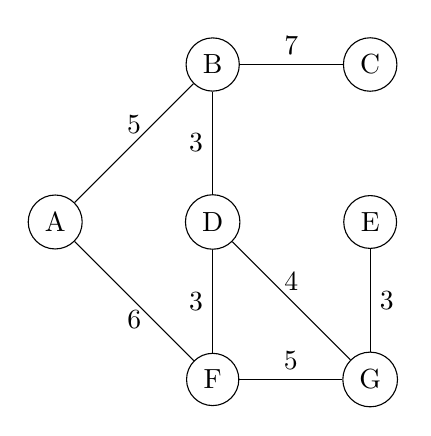
\begin{tikzpicture}
        % Nodi
        \node[circle, draw] (A) at (0,0) {A};
        \node[circle, draw] (B) at (2,2) {B};
        \node[circle, draw] (D) at (2,0) {D};
        \node[circle, draw] (F) at (2,-2) {F};
        \node[circle, draw] (C) at (4,2) {C};
        \node[circle, draw] (G) at (4,-2) {G};
        \node[circle, draw] (E) at (4,0) {E};
    
        % Archi
        \draw[-] (A) -- (B) node[midway, above] {5}; % Arco da A a B
        \draw[-] (A) -- (F) node[midway, below] {6}; % Arco da B a D
        \draw[-] (B) -- (D) node[midway, left] {3}; % Arco da D a C
        \draw[-] (D) -- (F) node[midway, left] {3}; % Arco da C a A
        \draw[-] (B) -- (C) node[midway, above] {7}; % Arco da C a A
        \draw[-] (D) -- (G) node[midway, above] {4}; % Arco da C a A
        \draw[-] (F) -- (G) node[midway, above] {5}; % Arco da C a A
        \draw[-] (G) -- (E) node[midway, right] {3}; % Arco da C a A
    
    \end{tikzpicture}
\end{center}

I vari algoritmi che presenteremo differiscono per come rispondono alla domanda: "\textit{Dato che ho ispezionato il nodo, proseguo o vado indietro?}"


\subsection{Ricerca Non Informata}
\subsubsection{Depth-First-Search}
Un algoritmo classico di ricerca su grafo è la ricerca in profondità. In questa versione, la DFS è dotata di \textit{Backtracking}. Possiamo 
dire in generale che l'approccio di questo algoritmo è aggressiva, poichè ricerca subito in profondità la soluzione (potrebbe metterci molto o potrebbe metterci poco), ossia non c'è garanzia.
Inoltre possiamo osservare che gli alberi generati dalla DFS sono stretti e lunghi.\\
\smallskip
\textbf{Funzionamento:}
\begin{enumerate}
    \item Si parte dal nodo iniziale A (che sarà poi radice dell'albero finale)
    \item Se il nodo da esplorare ha dei figli, si aggiungono all'albero i vari figli; in caso ve ne sia più di uno,
    un \textit{Tie-Breaker} spesso usato è basato sull'ordine lessicografico (quindi, per esempio, se esploriamo A, il primo figlio da esplorare sarà B)
    \item Si torna indietro se: il nodo è foglia, oppure se il nodo è già stato visitato
\end{enumerate}

\textbf{Analisi}:
\begin{itemize}
    \item \textbf{Correttezza}: La dfs restituisce sempre un albero (grazie all'uso del Backtracking e all'eliminazione dei loop)
    \item \textbf{Completezza}: La dfs restituisce sempre un albero in cui un ramo contiene lo stato obiettivo (se esiste il percorso)
    \item \textbf{Complessità Temporale}: Dato b il \textit{Branching Factor} e d la \textit{profondità massima}, la complessità di tale algoritmo è esponenziale, ossia $O(b^d)$
    \item \textbf{Complessità Spaziale}: La memoria usata è quella necessaria per generare l'albero; in questo caso la complessità è $O(d)$ ossia la profondità massima del percorso dallo start al goal.

\end{itemize}

\subsubsection{Breath-First-Search}
Un altro algoritmo classico di ricerca su grafo è la ricerca in ampiezza. Anche la BFS è dotata di \textit{Backtracking}. Possiamo 
dire in generale che l'approccio di questo algoritmo è conservativa, poichè ricerca sempre allo stesso livello, garantendo di visitare tutti i nodi.
Possiamo inoltre dire che gli alberi generati dalla BFS sono larghi e corti.\\
\smallskip
\textbf{Funzionamento:}
\begin{enumerate}
    \item Si parte dal nodo iniziale A (che sarà poi radice dell'albero finale)
    \item Se il nodo padre ha dei figli da esplorare, vengono tutti aggiunti all'albero; Si prosegue poi ai figli del primo nodo figlio e così via.
    Il \textit{Tie-Breaker} che possiamo usare è ancora quello basato sull'ordine lessicografico.
    \item Si torna indietro se: il nodo è foglia, oppure se il nodo è già stato visitato
\end{enumerate}

\textbf{Analisi}:
\begin{itemize}
    \item \textbf{Correttezza}: Per lo stesso motivo della DFS
    \item \textbf{Completezza}: Per lo stesso motivo della DFS
    \item \textbf{Complessità Temporale}: Dato b il \textit{Branching Factor} e q la \textit{profondità minima}, la complessità di tale algoritmo è esponenziale, ossia $O(b^q)$ (quindi sempre minore, nel caso peggiore, della DFS)
    \item \textbf{Complessità Spaziale}: In questo caso, dato che non viene allocata altra memoria se non il grafo stesso, la complessità spaziale sarà $O(n)$ con n il numero di nodi. 
\end{itemize}
\subsubsection{DFS/BFS Ottimizzati}
Gli ultimi 2 algoritmi possono essere ottimizzati introducendo nuove strutture dati, usate per evitare di rivisitare 
i nodi e quindi per generare alberi più piccoli:

\paragraph{EQL (Enqueued List).}
La EQL, anche detta \textit{lista di accodamento}, è una lista che tiene traccia di tutti i nodi già visitati; è detta
di accodamento perchè ad ogni nuova visita, il nodo visitato viene aggiunto alla fine; quando si deve vistare un nodo
si verifica che questo non sia già nella lista; se lo è, tutto il sottoalbero relativo non verrà esplorato. Questa 
operazione è detta \textbf{Potatura} o \textbf{Pruning}

\paragraph{Frontiera.}
Definiamo frontiera l'insieme dei nodi foglia non ancora espansi dell'albero; è detta così dal momento che, per la
\textbf{Separation Property}, separa la parte dell'albero esplorata da quella ancora non esplorata.\\
Implementazioni della Frontiera:
\begin{itemize}
    \item \textbf{Caso BFS}: la frontiera viene implementata come \textbf{Queue} (una coda FIFO)
    \item \textbf{Caso DFS}: la frontiera viene implementata come \textbf{Stack} (una coda LIFO)
\end{itemize}

\textbf{Analisi}:
\begin{itemize}
    \item \textbf{Correttezza}: L'uso delle EQL pota solo i sottoalberi già esplorati, per cui la correttezza non viene compromessa
    \item \textbf{Completezza}: L'algoritmo è ancora completo per il motivo precedente
    \item \textbf{Complessità Temporale/Spaziale}: anche se abbiamo introdotto queste strutture dati per ottimizzare le operazioni,
          in realtà la complessità nel caso peggiore non cambia. Grazie a queste ottimizzazioni, tuttavia, è possibile usare in un tempo ragionevole
          i 2 algoritmi
\end{itemize}

\newpage
\subsection{Proprietà dei Segnali}
\subsubsection{Durata}
La durata di un segnale è, considerando un segnale nel tempo, la differenza tra il primo istante in cui il segnale non è nullo e l'ultimo istante.

\subsubsection{Area}
Si dice \textit{Area di un Segnale} $s(t)$ l'area sottesa dallo stesso segnale, ossia:
\begin{equation}
    \int_{-\infty}^{+\infty} s(t)dt
\end{equation}

\subsubsection{Valor Medio (o Media Temporale)}
Il valor medio di un segnale $s(t)$ non è altro che quel valore $\tilde{s}$ tale che una funzione costante $s'(t) = \tilde{s}$ ha la stessa area di $s(t)$, ossia:
\begin{equation}
    \tilde{s} = \lim_{T \rightarrow +\infty} \frac{1}{2T} \int_{-T}^{+T}s(t)dt
\end{equation}

\subsubsection{Energia}
Sebbene non stiamo parlando propriamente di lavoro e concetti fisici relativi, dobbiamo dire che un segnale è sempre associato ad una certa energia che il segnale stesso trasporta.
Dunque \textit{l'energia di un segnale $(s(t))$} è:
\begin{equation}
    E_s = \int_{-\infty}^{+\infty} |s(t)|^2 dt
\end{equation}

\subsubsection{Potenza Istantanea}
Per il discorso precedente, possiamo anche definire la Potenza Istantanea di un segnale (cioè la potenza in un istante del Segnale) come
\begin{equation}
    P[s(t)] = \begin{cases}
        s(t_0)\overline{s(t_0)} & \mbox{ se } s(t_0) \in \mathbb{C} \\
        s(t_0)^2 & \mbox{ se } s(t_0) \in \mathbb{R}
    \end{cases}
\end{equation}

\subsubsection{Potenza Media}
La potenza media possiamo, invece, vederla come il valore medio dell'energia, ossia:
\begin{equation}
    P_s = \lim_{T \rightarrow +\infty} \frac{1}{2T} \int_{-T}^{+T}|s(t)|^2 dt
\end{equation}

\subsubsection{Segnale Energia e Potenza} \label{def: sep}
Innanzitutto possiamo notare come sia Potenza Media che Energia siano non negativi per costruzione;
inoltre tra Potenza Media e Energia di un segnale è possibile vedere una correlazione: laddove l'energia del segnale è finita, allora la potenza è necessariamente nulla;
laddove invece la potenza media è maggiore di 0, l'energia è infinita.

In base a questo concetto è possibile definire:
\begin{itemize}
    \item \textbf{Segnale Energia} un segnale $s(t)$ se e solo se $0 < E_s < \infty$ e allora $P_s = 0$
    \item \textbf{Segnale Potenza} un segnale $s(t)$ se e solo se $0 < P_s < \infty$ e allora $E_s \rightarrow +\infty$
\end{itemize}

\newpage

\section{Segnali Discreti}
A differenza dei segnali continui, i segnali discreti sono funzioni con Dominio discreto, solitamente rappresentate nella seguente maniera:
\begin{equation*}
    y = f(n), \mbox{  } n \in Z
\end{equation*}
Enunciamo ora tutte le proprietà, in maniera speculare, che abbiamo già descritto per i segnali continui:
\subsection{Operazione sui Segnali Discreti}
\subsubsection{Traslazione}
Dato un segnale $y = f(n)$ definiamo $y' = f(n - n_0)$ traslazione in avanti di $n_0$; definiamo invece $y'' = f(n + n_0)$ traslazione indietro di $n_0$.
\subsubsection{Decimazione/UpSampling}
Dato $y=f(n)$ il segnale con $n \in \mathbb{Z}$, il segnale decimato è:
\begin{equation}
    y = f(an) \mbox{ con } a \in Z \mbox{ e } |a| \geq 1 
\end{equation}
Questa operazione è detta \textit{decimazione} dal momento che è come se prelevassi selettivamente i valori ogni $a$ campioni del segnale di partenza

\subsubsection{Interpolazione/DownSampling}
Dato $y=f(n)$ il segnale con $n \in \mathbb{Z}$, il segnale interpolato è:
\begin{equation}
    y = f\left(\frac{n}{a}\right) \mbox{ con } a \in Z \mbox{ e } |a| \geq 1 
\end{equation}
In parole povere, questa operazione non fa altro che distanziare ogni campione di $a$ intervalli.

\newpage

\subsection{Segnali Notevoli}
\subsubsection{Rettangolo Discreto}
Viene definito come:
\begin{equation}
    rect\left(\frac{n}{D}\right) = \begin{cases}
        1 & \mbox{ se } |\frac{n}{D}| \leq \frac{1}{2}\\
        0 & \mbox{ altrimenti}
    \end{cases}
\end{equation}
\begin{center}
    \begin{tikzpicture}
        % Assi
        \draw[->] (-4,0) -- (4,0) node[below] {$n$}; % asse del tempo discreto
        \draw[->] (0,-2) -- (0,2) node[left] {$rect\left(\frac{n}{D}\right)$}; % asse dell'ampiezza
    
        
        \draw[dashed] (-2,0) -- (-2,1);
        \filldraw[blue] (-2,1) circle (2pt);
        
        \draw[dashed] (-1,0) -- (-1,1);
        \filldraw[blue] (-1,1) circle (2pt);
    
        \draw[dashed] (0,0) -- (0,1);
        \filldraw[blue] (0,1) circle (2pt);
    
        \draw[dashed] (1,0) -- (1,1);
        \filldraw[blue] (1,1) circle (2pt);
    
        \draw[dashed] (2,0) -- (2,1);
        \filldraw[blue] (2,1) circle (2pt);
    
        \filldraw[blue] (-3,0) circle (2pt);
        \filldraw[blue] (3,0) circle (2pt);
        \filldraw[blue] (-4,0) circle (2pt);
        \filldraw[blue] (4,0) circle (2pt);
    
    
    
        % Etichettatura degli intervalli di campionamento
        \draw (-2,0) node[below] {$-\frac{D}{2}$};
        \draw (2,0) node[below] {$\frac{D}{2}$};
        \draw (0,1) node[left] {$1$};
    \end{tikzpicture}
\end{center}

\subsubsection{Gradino Unitario}
Anche in questo caso, la formulazione è identica al Gradino Unitario continuo, ossia:
\begin{equation}
    u(t) = \begin{cases}
        1 & \mbox{ se } n \geq 0\\
        0 & \mbox{ se } n < 0
    \end{cases} 
\end{equation}

\subsubsection{Impulso Discreto}
Questo segnale è il parente "discreto" della \textit{Delta di Dirac} (\ref{eq:delta}) ma è più semplice da introdurre, dal momento che la sua formula è:
\begin{equation}
    \delta(n) = \begin{cases}
        1 & \mbox{ se } n = 0\\
        0 & \mbox{ se } n \neq 0
    \end{cases}
\end{equation}
Possiamo dunque notare che, a differenza della delta, l'impulso discreto è una vera e propria funzione.

\subsubsection{Proprietà dell'Impulso Discreto}
\begin{itemize}
    \item \textbf{Area Unitaria}: è abbastanza ovvia
    \begin{equation}
        \sum_{n=-\infty}^{+\infty} \delta(n) = 1
    \end{equation}

    \item \textbf{Prodotto Scalare con $\delta(n)$} 
    \begin{equation}
        \langle f,\delta \rangle = \sum_{n= -\infty}^{\infty} f(n)\delta(n) = f(0) 
    \end{equation}

    \item \textbf{Prodotto con $\delta(n)$}:
    \begin{equation}
        f(n)\delta(n - n_0) = f(n_0)\delta(n - n_0)
    \end{equation}

    \item \textbf{Integrazione Discreta}:
    \begin{equation}
        \sum_{i = -\infty}^{\infty} \delta(i) = \begin{cases}
            1 & \mbox{ se } n \geq 0\\
            0 & \mbox{ se } n < 0
        \end{cases} = u(n)
    \end{equation}
\end{itemize}

\subsubsection{Segnali Periodici Discreti}
Dato $s(n)$ un segnale con $n \in \mathbb{Z}$ è periodico se e solo se
\begin{equation}
    s(n) = s(n + kN), \mbox{ con periodo }N, \forall n,k \in \mathbb{Z}
\end{equation}
Se $N$ è il periodo di $s(n)$, allora la frequenza sarà $\frac{1}{N}$; Dal momento che $|N| \geq 1$ sempre (non ha senso avere periodo nullo), allora la frequenza è sempre frazionaria.
Si può dimostrare che solo un segnale con frequenza razionale può essere periodico, mentre se è irrazionale non lo potrà mai essere.

\subsubsection{Fasore Discreto}
La funzione è molto simile al fasore continuo:
\begin{equation}
    s(n) = e^{2\pi j f_0 n}
\end{equation}
Dove $f_0$ dev'essere razionale altrimenti la funzione non sarà periodica.
\newpage
\subsection{Proprietà dei Segnali Discreti}
\subsubsection{Durata}
La durata di un segnale discreto è la somma delle "stecche" non nulle di un grafico, o meglio, la lunghezza del supporto di $s(t)$
\begin{equation}
    D = n_2 - n_1 + 1
\end{equation}
Dove $n_2,n_1$ sono gli estremi non nulli del segnale.

\subsubsection{Area}
Dato $s(n), n \in \mathbb{Z}$
\begin{equation}
    A = \sum_{n = -\infty}^{+\infty} s(n)
\end{equation}

\subsubsection{Valor Medio}
Il valor medio è un $\tilde{s}$ tale che la funzione costante $s(t)' = \tilde{s}$ ha la stessa area di $s(t)$
\begin{equation}
    \tilde{s} = \lim_{N \rightarrow +\infty} \frac{1}{2N + 1} \sum_{n=-N}^{+N} s(n)
\end{equation}

\subsubsection{Potenza Istantanea}
Non è altro che il modulo del segnale in un determinato istante $n$, ossia:
\begin{equation}
    P_s(n) = \begin{cases}
        s(n)\overline{s(n)} \mbox{ se } s(n) \in \mathbb{C} \\
        s(n)^2 \mbox{ altrimenti}
    \end{cases}
\end{equation}

\subsubsection{Energia}
è l'area della Potenza Istantanea, ossia:
\begin{equation}
    E_s = \sum_{n=-N}^{+N} |s(n)|^2
\end{equation}

\subsubsection{Potenza Media}
è il valor medio della Potenza Istantanea, ossia:
\begin{equation}
    P_s =  \lim_{N \rightarrow +\infty} \frac{1}{2N + 1} \sum_{n=-N}^{+N} |s(n)|^2
\end{equation}

\subsubsection{Segnali Potenza ed Energia}
Anche in questo caso possiamo fare la distinzione tra i segnali potenza e i segnali energia, la definizione è la stessa presentata 
alla sezione \eqref{def: sep}

\newpage

\section{Sistemi}
In forma generale, un sistema descrive una relazione/processo di Causa-Effetto tra un INPUT ed un OUTPUT. In particolare nel corso 
ci focalizzeremo sui sitemi di Elaborazione dei Segnali.\\
Un \textbf{Sistema di Elaborazione dei Segnali} può essere vista come una relazione o legge di trasformazione di un segnale in un altro,
dunque, formalmente:\\
Dato un sistema $S[\cdot]$, possiamo dire che:
\begin{equation}
    y(b) = S[x(t)]
\end{equation}
Dove $y(b)$è il segnale in output mentre $x(t)$ è il segnale in input.
In base alla continuità dei segnali e dei domini possiamo distinguere i sistemi in: \textbf{Continui, Discreti e Misti}

\subsection{Sistemi Continui}
Dato un sistema $y(b) = S[x(a)]$, con $b \in B, a \in A$ questo si dice continuo se e solo se:
\begin{itemize}
    \item $A,B$ sono insiemi continui
    \item $y(b),x(a)$ sono funzioni continue
\end{itemize}
Una classe importante di questi sistemi sono i \textbf{Sistemi Tempo-Continui} in cui la variabile è il tempo.

\paragraph{Esempi. }
\begin{itemize}
    \item \textbf{Ritardatori}
    \begin{equation}
        y(t) = S[x(t)] = x(t - t_0)
    \end{equation}
    Questo sistema non fa altro che ritardare il segnale $x(t)$ di una quantità di $t_0$ secondi.

    \item \textbf{Quantizzatore}
    \begin{equation}
        y(t) = \mbox{ROUND}(x(t))
    \end{equation}
    Questo sistema arrotonda ogni valore di $x(t)$ al suo intero più vicino.

    \item \textbf{Integratore}
    \begin{equation}
        y(t) = S[x(t)] = \int_{t - T}^{t} x(\tau)d\tau
    \end{equation}
    Questo sistema associa ad ogni istante $t$ l'area compresa tra $t - T$ e $t$
\end{itemize}

\subsection{Proprietà dei Sistemi Tempo-Continui}
\subsubsection{Non Dispersività}
Un sistema $S[\cdot]$ è non dispersivo se e solo se il sistema dipende solo da $t$ e dal valore attuale di $x(t)$, ossia:
\begin{equation}
    y(t) = S[t; x(t)]
\end{equation}
possiamo dire che questi sistemi sono senza memoria perchè non considerano per nulla il passato.
\paragraph{Esempio:}
\textbf{Amplificatore Ideale}
\begin{equation}\label{eq: AmpId}
    y(t) = A \cdot x(t)
\end{equation}

\subsubsection{Causalità}
Un sistema $S[\cdot]$ è causale se e solo se:
\begin{equation}
    y(t) = S[t; x(\tau) \mbox{ dove } \tau \leq T]
\end{equation}
Questi sistemi associano ad ogni istante t un valore dipendente non soltanto dal tempo attuale e dal valore $x(t)$, ma 
anche della storia di $x(t)$. Bene o male tutti i sistemi reali sono causali, perchè dipendono anche dagli istanti passati di un segnale.
Esistono (ma solo in teoria) i segnali \textbf{Anticausali}, in cui il sistema dipende dall'istante attuale e quelli futuri (e quindi il futuro causerebbe il presente, impossibile nella realtà)

\subsubsection{Stabilità BIBO (Bounded Input, Bounded Output)}
Un sistema è \textbf{Stabile} se e solo se per ogni input limitato, l'uscita è sempre limitata, ossia:\\
Dato $S[\cdot]$ dove $y(t) = S[x(t)]$ con $|x(t)| \leq K_x < +\infty$  $\forall t \in \mathbb{R}$ allora:
\begin{equation}
    |y(t)| \leq K_y < +\infty \mbox{  } \forall t \in \mathbb{R}
\end{equation}
Dove $K_x,K_y$ sono rispettivamente il limite superiore/inferiore di $x(t),y(t)$
\paragraph{Esempi:} L'Amplificatore Ideale \eqref{eq: AmpId}.
\subsubsection{Omogeneità}
Dato un sistema $S[\cdot] : y(t) = s[x(t)]$, $S$ è detto \textit{omogeneo} se e solo se vale questa proprietà:\\
Dato come input $a\cdot x(t)$ con $a \in \mathbb{R}$ allora:
\begin{equation}
    S[a\cdot x(t)] = a\cdot y(t)
\end{equation}

\subsubsection{Additività}
Dato un sistema $S[\cdot] : y(t) = s\left[x(t)\right]$, $S$ è detto \textit{additivo} se e solo se vale questa proprietà:\\
Dato come input $x(t) = \sum_{i = 1}^{N} x_i(t)$ allora:
\begin{equation}
    S[x(t)] = S\left[\sum_{i = 1}^{N} x_i(t)\right] = \sum_{i = 1}^{N} y_i(t)
\end{equation}

\subsubsection{Linearità}
Un sistema $S[\cdot] : y(t) = s\left[x(t)\right]$ è detto \textit{lineare} se è sia omogeneo che additivo con gli stessi pesi, ossia se:\\
Dato $x(t) = \sum_{i = 1}^{N} a_i x_i(t)$ allora:
\begin{equation}
    S[x(t)] = S\left[\sum_{i = 1}^{N} a_i x_i(t)\right] = \sum_{i = 1}^{N} a_i y_i(t)
\end{equation}
Questa proprietà è dovuta, nei segnali, al \textit{Principio di sovrapposizione degli Effetti}, ossia:\\
\textit{La risposta di un sistema ad una combinazione lineare degli ingressi è uguale alla combinazione lineare con gli stessi
coefficienti delle risposte ad ogni singolo ingresso}

\paragraph{Esempi.}
\begin{itemize}
    \item \textbf{Integratore definito nel tempo}: grazie alla proprietà di linearità dell'integrale, questo sistema è lineare:
    \begin{equation}
        y(t) = \int_{t -T}^{t} \sum_{i = 1}^{N} a_i x_i(\tau) d\tau = \sum_{i = 1}^{N}  \int_{t -T}^{t}  a_i x_i(\tau) d\tau = \sum_{i = 1}^{N} a_i y_i(t)
    \end{equation}
\end{itemize}


\subsubsection{Tempo-Invarianza}
Dato un sistema $S[\cdot] : y(t) = S[x(t)]$ tempo-continuo, S è tempo-invariante se e solo se:\\
\begin{equation}
    se S[x(t - t_0)] = y(t - t_0) \mbox{   } \forall t_0 \in \mathbb{R}
\end{equation}
Questa proprietà afferma che il sistema non dipende da un eventuale ritardo(o anticipo) del segnale.


\section{Sistemi Lineari e Tempo Invarianti (LTI)}
Sia la linearità che la tempo invarianza sono così importanti che dedicheremo un intero capitolo ai sistemi LTI (o Lineari e Tempo-Invarianti), dal momento
che tali proprietà implicano altre proprietà altrettanto interessanti, come quella legata alla risposta all'impulso.
Riprendiamo la proprietà \eqref{eq: camp} della delta di Dirac e un segnale $x(t)$. Consideriamo ora il sistema
\begin{equation*}
    S\left[\int_{\mathbb{R}}x(\tau)\delta(t - \tau) d\tau\right]
\end{equation*}
Se $S[\cdot]$ è lineare possiamo considerare $x(\tau)$ come coefficiente e ottenere:
\begin{equation}
    \int_{\mathbb{R}}x(\tau) S\left[\delta(t - \tau) \right]d\tau
\end{equation}
Possiamo definire la \textit{risposta all'impulso da parte del sistema} come $h(t) := S[\delta(t)]$.
Se S è anche tempo-invariante, allora
\begin{equation}
    h(t - t_0) = S[\delta(t - t_0)]
\end{equation}
Possiamo riscrivere l'equazione di partenza se $S[\cdot]$ è lineare e tempo-invariante come:
\begin{equation}
    x(t) = \int_{\mathbb{R}}x(\tau)h(t - \tau) d\tau
\end{equation}

\subsection{Prodotto/Integrale di Convoluzione}
Definiamo:
\begin{equation}
    x(t) \ast h(t) = \int_{-\infty}^{+\infty} x(\tau)h(t - \tau) d\tau
\end{equation}
E si dice \textit{x(t) convoluto con h(t)}; è un'operazione molto importante in segnali, tanto da avere una definizione.
L'importanza di $h(t)$ noi la possiamo apprezzare quando dobbiamo studiare un segnale ignoto: passando al sistema un impulso, 
e osservando l'output, tale output sarà proprio x(t) convoluto con h(t) (se il sistema è lineare e tempo invariante).
\subsubsection{Proprietà}
\begin{itemize}
    \item \textbf{Commutativa:}dati 2 segnali $f,g$
    \begin{equation} \label{prop: convComm}
        f(t) \ast g(t) = g(t) \ast f(t)
    \end{equation}
    Tale proprietà è facile da dimostrare:\\
    Consideriamo la convoluzione $f(t) \ast g(t) = \int_{-\infty}^{+\infty} f(\tau)g(t - \tau) d\tau$. Effettuiamo ora un cambio di variabile:
    \begin{equation*}
        \begin{cases}
            x = t - \tau\\
            \tau = t - x\\
            dx = -d\tau
        \end{cases}
    \end{equation*}
    Sostituiamo ora le $\tau$ per avere un integrale in $x$ (NB: gli estremi di integrazione si invertono dal momento che $x$ è un "ribaltamento" di $\tau$):
    \begin{align*}
        \int_{-\infty}^{+\infty} f(\tau)g(t - \tau) d\tau= \\
        \int_{+\infty}^{-\infty} f(t - x)g(x) (-dx) = \\
        \int_{-\infty}^{+\infty} g(x)f(t - x) dx = \\
        g(t) \ast f(t)
    \end{align*}
    Alla fine ho risolto il $-dx$ semplicemente invertendo ancora gli estremi di integrazione. Il significato di questa proprietà è importante:
    se è vero che è possibile studiare un sistema LTI rispetto alla sua risposta all'impulso, è vero anche il contrario, è possibile studiare un sistema rispetto ad un segnale $x(t)$
    \item \textbf{Associativa}: dati 3 segnali $f,g,h$ allora:
    \begin{equation}
        f(t) \ast [g(t) \ast h(t)] = [f(t) \ast g(t)] \ast h(t)
    \end{equation}

    \item \textbf{Distributiva (rispetto alla somma)}: dati 3 segnali $f,g,h$: \label{prop: ConvDistr}
    \begin{equation}
        f(t) \ast [g(t) + h(t)] = f(t) \ast g(t) + f(t) \ast h(t) 
    \end{equation}

    \item \textbf{Durata della Convoluzione}: \label{prop: ConvDurata} dati 2 segnali $f,g$ con durata rispettivamente $D_1,D_2$ allora la durata di $f(t) \ast g(t)$ è $D_1 + D_2$
    
    \item \textbf{Convoluzione con $\delta(t)$}: \label{prop: ConvDelta} dato un segnale $f(t)$ allora:
    \begin{equation}
        f(t) \ast \delta(t - t_0) = f(t - t_0)
    \end{equation}
    Possiamo infatti dire che $\delta(t)$ è l'operatore neutro dell'operazione di convoluzione, questo perchè il delta è una funzione che avviene tutta in un istante e quindi non altera la funzione di partenza; una sua eventuale traslazione, trasla la funzione $f(t)$.
    La dimostrazione è banale perchè si basa sulla proprietà del campionamento della delta \eqref{eq: camp}
\end{itemize}


\newpage

\subsection{Proprietà dei Sistemi LTI Continui}
\subsubsection{Causalità} \label{prop: causalita}
Dato un sistema LTI $S[\cdot] : y(t) = S[x(t)]$, $S$ è causale se $y(t)$ accade DOPO il segnale $x(t)$, questo per il concetto stesso di causalità:
$y(t)$ è la risposta all'impulso di $x(t)$ quindi DEVE accadere dopo, in particolare si dice che:\\
\begin{equation}
    \mbox{Un sistema è causale} \Longleftrightarrow h(t) = 0 \mbox{  } \forall t < 0
\end{equation}
Proprio per questo motivo, dal momento che $y(t)$ può essere descritto come risposta all'impulso, ossia come convoluzione tra $x(t)$ e $h(t)$, se 
il sistema è causale allora possiamo ridefinire la $y(t)$ come integrale dall'infinito passato fino all'istante $t$ presente, ossia:
\begin{equation}
    y(t) = \int_{-\infty}^{t} x(\tau) h(t - \tau) d\tau
\end{equation}
Possiamo anche, per la proprietà commutativa \eqref{prop: convComm}, riscrivere la $y(t)$ come integrale tra la risposta $h(t)$ e il segnale $x(t)$ ribaltato e traslato
di tutti i valori di $\tau$ da 0 fino all'infinito futuro
\begin{equation}
    y(t) = \int_{0}^{+\infty} h(\tau)x(t - \tau) d\tau
\end{equation}

\subsubsection{Stabilità BIBO} \label{prop: BIBO}
Dato un sistema LTI $S[\cdot] : y(t) = S[x(t)]$, $S[\cdot]$ è BIBO se e solo se:
\begin{equation}
    \forall x(t) : |x(t)| < M < \infty \rightarrow |y(t)| < N < \infty
\end{equation}
In particolare possiamo osservare che:
\begin{equation*}
    |y(t)| = |S[x(t)]| = \left|\int_{-\infty}^{+\infty} h(\tau) x(t - \tau) d\tau \right|
\end{equation*}
Sappiamo inoltre che, data una qualsiasi $f(x)$ vale questa disuguaglianza:
\begin{equation*}
    \left|\int_{-\infty}^{+\infty} f(x)dx \right| \leq \int_{-\infty}^{+\infty} |f(x)|dx
\end{equation*}
Dunque
\begin{equation*}
    y(t) \leq \int_{-\infty}^{+\infty} |h(\tau) x(t - \tau)|d\tau
\end{equation*}
Per la proprietà del valore assoluto $|ab| = |a||b|$ allora:
\begin{equation*}
    \int_{-\infty}^{+\infty} |h(\tau) x(t - \tau)|d\tau = \int_{-\infty}^{+\infty} |h(\tau)| |x(t - \tau)|d\tau
\end{equation*}
Ma $x(t - \tau) \leq M$ perchè abbiamo ipotizzato che il segnale in ingresso sia limitato, dunque
\begin{equation*}
    \int_{-\infty}^{+\infty} |h(\tau)| |x(t - \tau)|d\tau \leq M\int_{-\infty}^{+\infty} |h(\tau)|d\tau
\end{equation*}
In definitiva:
\begin{equation*}
    y(t) \leq M\int_{-\infty}^{+\infty} |h(\tau)|d\tau
\end{equation*}
Possiamo dunque affermare che condizione necessaria e sufficiente affinchè un sistema sia stabile BIBO è che $\int_{-\infty}^{+\infty} |h(\tau)|d\tau$ converga, altrimenti $y(t)$ è illimitato.\\
\paragraph{Teorema.} Se la risposta all'impulso del Sistema non è assolutamente convergente allora non è BIBO Stabile
\paragraph{Ipotesi. } Ipotizziamo che:
\begin{enumerate}
    \item Il sistema sia BIBO Stabile, $|y(t)| < N < \infty$
    \item $\int_{-\infty}^{+\infty} |h(\tau)| \tau = + \infty$
    \item consideriamo una $x(t)$ limitata, ossia $x(t) = \mbox{sign}[h(-t)]$ 
\end{enumerate}
\paragraph{Dimostrazione. } Possiamo dire che per $t = 0$ la risposta all'impulso è:
\begin{align*}
    &y(t) = \int_{-\infty}^{+\infty} h(\tau) x(0 -\tau) d\tau =  \int_{-\infty}^{+\infty} h(\tau)\mbox{sign}[h(-\tau)] d\tau
\end{align*}
per $t = 0$, $\mbox{sign}[h(-\tau)] = 1$ dunque:
\begin{equation*}
    \int_{-\infty}^{+\infty} h(\tau)\mbox{sign}[h(-\tau)] d\tau = \int_{-\infty}^{+\infty} h(\tau) d\tau
\end{equation*}
Inoltre
\begin{align*}
    \int_{-\infty}^{+\infty} h(\tau) d\tau &\leq \int_{-\infty}^{+\infty} |h(\tau)| d\tau = |y(t)| \\
    |y(t)| &= \int_{-\infty}^{+\infty} |h(\tau)| d\tau = \infty
\end{align*}
ASSURDO, allora $y(t)$ è instabile.\\Possiamo dunque affermare che:
Un sistema è BIBO se e solo se:
\begin{equation}
    \int_{-\infty}^{+\infty} |h(\tau)| d\tau < \infty
\end{equation}

\subsubsection{Risposta in frequenza}
Consideriamo la risposta del sistema rispetto al fasore di frequenza $f$:
\begin{equation*}
    x_f(t) = e^{j2\pi ft}
\end{equation*}
Dal momento che il sistema è LTI allora:
\begin{align*}
    y(t) = h(t) \ast x_f(t) = \\
    = \int_{-\infty}^{+\infty} h(\tau)e^{j2\pi f(t - \tau)} d\tau =\\
    = \int_{-\infty}^{+\infty} h(\tau)e^{j2\pi ft}e^{-j2\pi\tau} d\tau =\\
    = e^{j2\pi ft} \int_{-\infty}^{+\infty} h(\tau) e^{-j2\pi\tau} d\tau 
\end{align*}
\begin{highlightedeq}
    Possiamo vedere $\int_{-\infty}^{+\infty} h(\tau) e^{-j2\pi\tau} d\tau$ come una sorta di convoluzione in 0, che noi chiamiamo $H(f)$ 
    e definiamo \textbf{Risposta in Frequenza}. Possiamo riscrivere l'equazione come:
    \begin{equation}
        y(t) = H(f)x_f(t)
    \end{equation}
\end{highlightedeq}
Da $H(f)$ possiamo definire:
\begin{itemize}
    \item \textbf{Risposta in Ampiezza}: $|H(f)|$
    \item \textbf{Risposta in Fase}: $\angle H(f)$
\end{itemize}
Questa proprietà dei LTI è molto importante poichè ci dice che la risposta in frequenza di un qualsiasi segnale $x(t)$ è un altro segnale \textbf{alla stessa frequenza}, magari traslato o amplificato,
cioè la risposta di un fasore è ancora un fasore di frequenza $f$ ma moltiplicato per un valore complesso $H(f)$



\subsection{Proprietà Sistemi Discreti}
Un sistema $S[\cdot]:y(t) = S[x(t)]$ è detto discreto se e solo se $x,y$ sono segnali discreti; possiamo enunciare per tali sistemi le stesse proprietà dei sistemi LTI continui:
\paragraph{Causalità.}
Ha la medesima formulazione dei sistemi LTI Continui \eqref{prop: causalita} 

\paragraph{Stabilità BIBO.}
Ha la medesima formulazione dei sistemi LTI Continui \eqref{prop: BIBO} 

\paragraph{Linearità.}
Ha la medesima formulazione dei sistemi LTI Continui \eqref{prop: linearita} 

\paragraph{Tempo-Invarianza.} 
La medesima formulazione dei sistemi LTI Continui \eqref{prop: TI} 
\subsection{Ottimizzazioni di Minimax}
\subsubsection{$\alpha,\beta$ Pruning}
Sebbene l'algoritmo Minimax appena presentato sia corretto e completo, è evidente la sua inefficienza per 2 motivi:
\begin{itemize}
    \item L'algoritmo deve sempre attraversare tutto l'albero per ottenere il \textit{valore di gioco}
    \item In caso di alberi di grandi dimensioni, la complessità cresce notevolmente
\end{itemize}
Così come abbiamo fatto per gli algoritmi di ricerca, è possibile ottimizzare Minimax potando alcuni sottoalberi e risparmiando
dunque tempo di computazione (NB: nonostante ciò, la complessità dell'algoritmo rimane esponenziale).


\paragraph{Algoritmo.}Per potare i vari sottoalberi, l'algoritmo deve assegnare ad ogni nodo dell'albero una coppia di valori $\left[\alpha, \beta\right]$:
\begin{itemize}
    \item $\alpha$ rappresenta il \textbf{minimo valore garantito} per il giocatore \textbf{MAX} ad un certo nodo dell'albero
    \item $\beta$ rappresenta il \textbf{massimo valore garantito} per il giocatore \textbf{MIN} ad un certo nodo dell'albero
\end{itemize}
Durante \textbf{l'esplorazione} dell'albero:
\begin{itemize}
    \item Quando un nodo viene esplorato per la \textbf{prima volta}, l'algoritmo gli assegna i valori $\left[-\infty,+\infty\right]$, poi:
    \begin{itemize}
        \item Se il nodo da esplorare è un nodo MAX, viene aggiornato il suo valore di $\alpha$ con il valore più alto dei suoi sottoalberi
        \item Se il nodo da esplorare è un nodo MIN, viene aggiornato il suo valore di $\beta$ con il valore più basso dei suoi sottoalberi
    \end{itemize}
    \item Quando un nodo viene \textbf{completamente esplorato} allora vale che: $\alpha = \beta$.
    \item Invece, se si scopre che il nodo \textbf{appena esplorato} presenta un valore $v$ che è:
    \begin{itemize}
        \item $v < \alpha$ se il padre è un nodo \textbf{MAX}
        \item $v > \beta$ se il padre è un nodo \textbf{MIN}
    \end{itemize}
    Allora tutti gli altri sottoalberi del nodo padre vengono \textbf{potati} e non esplorati.
\end{itemize}


\paragraph{Analisi}
L'efficacia del pruning, dunque, dipende molto dallo scoprire le \textit{"killer moves"}, ossia dei valori $\alpha,\beta$ stringenti per la potatura dei sottalberi. 
Se i valori più stringenti si trovano solo alla fine dell'esplorazione, il pruning non è più apprezzabile e la computazione risparmiata è minima.
Valutiamo, in particolare, la complessità nei 2 casi:
\begin{itemize}
    \item \textbf{Caso Pessimo}: i valori stringenti $\alpha,\beta$ di un nodo vengono scoperti negli ultimi sottoalberi, per cui non vi è alcuna potatura (stessa complessità di una DFS $O(b^d)$ (vedi \ref{alg: dfs}))
    \item \textbf{Caso Ottimo}: Per ogni nodo MAX, tutti i suoi alberi vengono esplorati, mentre per ogni nodo MIN, il primo sottoalbero fornisce già i valori $\alpha,\beta$ per il pruning di tutti gli altri sottoalberi,
    dunque, è possibile dimostrare, che la complessità è $O(b^{d/2})$, ossia che nello stesso tempo, un MINIMAX con pruning esplora il quadrato dei nodi di un semplice MINIMAX
\end{itemize}
Rimane dunque evidente il fatto che per la maggior parte dei giochi è \textbf{impossibile} esplorare l'albero di gioco e trovare sempre, 
in tempo ragionevole, il valore di gioco; anzi, se lo fosse, il gioco non sarebbe più interessante (come il tris). Inoltre Minimax risulta essere poco utile quando il tempo per decidere
una mossa risulta essere molto limitato.
\paragraph{Esiti di una partita.} In generale possiamo dire che una partita tra 2 intelligenze artificiali A e B può concludersi in uno dei seguenti modi:
\begin{itemize}
    \item A si arrende
    \item B si arrende
    \item A e B patteggiano
\end{itemize} 

\subsubsection{Funzioni di Valutazione e CUTOFF}
Un problema sicuramente noto del pruning $\alpha,\beta$ è che per trovare un valore $\alpha$ o $\beta$, l'algoritmo deve arrivare fino ad una foglia
dell'albero, cosa assolutamente impossibile per alberi di gioco davvero grandi (come gli scacchi o il go). Un'intuizione che propose Shannon
verso la fine degli anni '50 fu quella di interrompere la valutazione di un nodo (se contiene troppi sottoalberi) e farlo diventare un nodo foglia
il cui valore è una stima della bontà del nodo calcolata da una \textbf{Funzione di Valutazione}, ossia un'euristica $v(s)$ con $s$ il nodo attuale.
La decisione di continuare ad esplorare un nodo non terminale tramite Minimax o approssimarlo tramite Funzione di valutazione viene fatta da un predicato 
(una funzione booleana), ossia CUT$(s,d)$ con $s$ il nodo attuale e $d$ la profondità massima di ricerca:
\begin{itemize}
    \item se CUT$(s,d) = $ TRUE, allora approssimo il valore del nodo con l'euristica $v(s)$
    \item altrimenti continuo ad esplorarlo tramite MINIMAX
\end{itemize}
Man mano che scendo nell'albero, il valore $d$ decrementa fino ad arrivare a $0$.
Una forma di euristica che è possibile realizzare per un gioco determina la bontà di un nodo attraverso la combinazione (lineare o non) delle \textit{caratteristiche}
di uno stato (per esempio, negli scacchi, una caratteristica di uno stato potrebbe essere la "presenza della regina", con peso 10, la "presenza di un alfiere", con peso 6, la "posizione dei pedoni", ecc...) (Pag. 237).

\paragraph{Iterative Deepening.} Una possibile implementazione di CUT è tramite la funzione di \textit{approfondimento iterativo} della DFS e consiste nell'incrementare $d$
ad ogni nuovo sottoalbero esplorato, cioè consiste nell'aumentare il \textit{budget di esplorazione} e a scommettere sempre di più su un ramo, scendendo via via più in profondità

\paragraph{Quiescient Search.} Un altro approccio utilizzabile per CUT risiede nel riconoscimento dei nodi \textbf{Quiescienti} e di quelli \textbf{Non Quiescenti}.
Un nodo è quiescente se non è \textit{interessante}, ossia una qualunque mossa non stravolge gli esiti del match; con questo approccio dunque, tutti gli stati potenzialmente quiescienti vengono approssimati,
mentre quelli più interessanti vengono esplorati con MINIMAX.

\newpage


\section{Analisi In Frequenza}
\lezione{Lezione 10}{29/10/2024}
I segnali visti finora sono stati presentati come funzioni descritte da un'espressione analitica; alcuni studiosi, tra cui Fourier,
si accorsero che tali funzioni potevano essere scomposte in somme di altre funzioni (in particolare di fasori, seni e coseni), ossia
è possibile vedere un segnale come \textbf{combinazione lineare} di segnali elementari. Uno strumento che permette di trasformare
un segnale in una combinazione lineare di segnali elementari è lo \textbf{sviluppo in serie di Fourier}.

\subsection{Sviluppo In Serie Di Fourier}
\begin{highlightedeq}
    \paragraph{Teorema.}Data una funzione \textit{periodica} $f(t) : f(t) = f(t + kT)$  $\forall t \in \mathbb{R}, k \in \mathbb{Z}$ e \textit{regolare}
    (ossia che rispetta le condizioni di Dirichlet), allora $f(t)$ piò essere riscritta come una combinazioni lineare di seni e 
    coseni con i propri pesi e le cui frequenze sono multiple di $\frac{1}{T}$ (con $T$ il periodo di $f(t)$).
\end{highlightedeq}

Consideriamo ora i vari multipli:
\begin{itemize}
    \item $n = 0 \longrightarrow f_0 = 0$ è la cosiddetta \textit{componente continua} (un valore costante).
    \item $n = 1 \longrightarrow f_1 = \frac{1}{T}$ viene detta la \textit{frequenza fondamentale}.
    \item $\forall |n| > 1 \longrightarrow f_n = \frac{n}{T}$ viene detta \textit{armonica n-esima}.
\end{itemize}

Gli sviluppi in serie di fourier si presentano in forma \textbf{Trigonometrica} ed \textbf{Esponenziale}

\subsubsection{Forma Esponenziale}
\paragraph{Equazione di Sintesi.}Nella forma esponenziale possiamo esprimere la funzione $f(t)$ come combinazione lineare di fasori \eqref{eq: fasore} $p_n(t)$ a
frequenza $f_n = \frac{1}{T}$ con $T$ il periodo di $f$; è detta \textit{di sintesi} perchè otteniamo $f$ dalla combinazione di fasori
\begin{equation}
    f(t) = \sum_{n = -\infty}^{+\infty} c_n e^{j2\pi \frac{n}{T} t}  \tag{$t \in \mathbb{R}$}
\end{equation}

\paragraph{Equazione di Analisi.} Al contrario della sintesi, noi vogliamo \textit{scomporre} $f$ per ottenere i fasori che la combinano:
\begin{equation}
    c_n = \frac{1}{T} \int_{T} f(t)e^{-j2\pi \frac{n}{T}t} dt \tag{$n \in \mathbb{Z}$}
\end{equation}
Dove $\int_{T}$ è un integrale \textit{di durata T}, ossia che può andare da $0$ a $T$, o da $-T/2$ a $T/2$

\subsubsection{Forma Trigonometrica}
Anche se storicamente è stato al contrario, possiamo derivare a partire dalla forma esponenziale, la forma trigonometrica dello sviluppo.
\paragraph{I Equazione di Sintesi}\begin{equation*}
    f(t) = \sum_{n = -\infty}^{+\infty} c_n e^{j2\pi \frac{n}{T} t} = c_0 + \sum_{n = -\infty}^{+\infty}[ c_n e^{j2\pi \frac{n}{T} t} + c_{-n} e^{-j2\pi \frac{n}{T} t}] \tag{separo i $c_n$}
\end{equation*}
Consideriamo ora $c_{-n}$
\begin{align*}
    c_{-n} =& \frac{1}{T} \int_{T} f(t)e^{-j2\pi \frac{n}{T}t} dt = \\
    =& \frac{1}{T} \int_{T} f(t)\overline{e^{j2\pi \frac{n}{T}t}} dt = \overline{c_n}
\end{align*}
Possiamo vedere il complesso $-j$ come il coniugato del complesso di partenza, dunque:
\begin{align*}
    f(t) =& c_0 + \sum_{n = -\infty}^{+\infty}[ c_n e^{j2\pi \frac{n}{T} t} + \overline{c_{n}} e^{-j2\pi \frac{n}{T}t }] =\\
         =& c_0 + \sum_{n = -\infty}^{+\infty}[ c_n e^{j2\pi \frac{n}{T} t} + \overline{c_{n} e^{j2\pi \frac{n}{T}t} }] = \\
         =& c_o + \sum_{n = -\infty}^{+\infty} 2\mathbb{R}e [c_n e^{j2\pi \frac{n}{T}t}] \tag{proprietà \ref{prop: coniugato}}
\end{align*}
Possiamo dunque notare che, a partire dalla scomposizione di una funzione reale in fasori (complessi) otteniamo ancora qualcosa di completamente reale.
Poniamo ora $c_n = \rho_n e^j \theta_n$, ossia in forma polare:
\begin{align*}
    f(t) &= c_o + \sum_{n = -\infty}^{+\infty} 2\mathbb{R}e [\rho_n e^{j \theta_n} e^{j2\pi \frac{n}{T}t}] =\\
         &= c_o + \sum_{n = -\infty}^{+\infty} 2\mathbb{R}e [\rho_n e^{j2\pi \frac{n}{T}t +\theta_n }] =
\end{align*}
Dal momento che $\mathbb{R}e[e^{j\theta}] = \cos(\theta)$ allora:
\begin{equation}
    f(t) = c_0 + 2 \int_{n = 1}^{+\infty} \rho_n \cos\left(2\pi \frac{n}{T}t +\theta_n\right)
\end{equation}

\paragraph{II Equazione di Sintesi.} Ora poniamo $c_n = a_n - jb_n$:
\begin{align*}
    f(t) =& c_o + \sum_{n = -\infty}^{+\infty} 2\mathbb{R}e \left[c_n e^{j2\pi \frac{n}{T}t}\right] =\\
         =& c_o + \sum_{n = -\infty}^{+\infty} 2\mathbb{R}e \left[(a_n - jb_n) e^{j2\pi \frac{n}{T}t}\right] =\\
         =& c_o + \sum_{n = -\infty}^{+\infty} 2\mathbb{R}e \left[a_n e^{j2\pi \frac{n}{T}t} - jb_n e^{j2\pi \frac{n}{T}t}\right] =\\
\end{align*}
Riscriviamo ora $j$ come $j = e^{j \frac{\pi}{2}}$:
\begin{equation*}
    f(t) = c_o + \sum_{n = -\infty}^{+\infty} 2\mathbb{R}e \left[a_n e^{j2\pi \frac{n}{T}t} - b_n e^{j2\pi \frac{n}{T}t + \frac{\pi}{2}}\right] =
\end{equation*}
Sapendo che, ancora una volta, $\mathbb{R}e[e^{j\theta}] = \cos(\theta)$ allora:
\begin{equation*}
    = c_o + 2\sum_{n = -\infty}^{+\infty} \left[a_n \cos\left(2\pi \frac{n}{T}t\right) - b_n \cos\left(2\pi \frac{n}{T}t + \frac{\pi}{2}\right)\right] =
\end{equation*}
Dal momento che $\cos\left(\theta + \frac{\pi}{2}\right) = -\sin(\theta)$ allora:
\begin{equation}
    f(t) = c_o + 2\sum_{n = -\infty}^{+\infty} \left[a_n \cos\left(2\pi \frac{n}{T}t\right) + b_n \sin\left(2\pi \frac{n}{T}t\right)\right]
\end{equation}
Cerchiamo, a questo punto, di derivare $a_n, b_n$ a partire da $c_n$:
\begin{align*}
    a_n &= \mathbb{R}e[c_n] = \mathbb{R}e\left[ \frac{1}{T} \int_{T} f(t) e^{-j2\pi \frac{n}{T} t} dt \right] =\\
        &= \frac{1}{T} \int_{T} f(t) \mathbb{R}e\left[e^{-j2\pi \frac{n}{T} t}\right] dt =\\
        &= \frac{1}{T} \int_{T} f(t) \cos\left(2\pi \frac{n}{T}t\right)dt
\end{align*}
\begin{align*}
    b_n &= -\mathbb{I}m[c_n] = -\mathbb{I}m\left[ \frac{1}{T} \int_{T} f(t) e^{-j2\pi \frac{n}{T} t} dt \right] =\\
        &= -\frac{1}{T} \int_{T} f(t) \mathbb{I}m\left[e^{-j2\pi \frac{n}{T} t}\right] dt =\\
        &= -\frac{1}{T} \int_{T} f(t) \sin\left(-2\pi \frac{n}{T}t\right)dt =       
\end{align*}
Per la proprietà antisimmetrica del seno $\sin(-\theta) = -\sin(\theta)$ otteniamo:
\begin{equation*}
   b_n = \frac{1}{T} \int_{T} f(t) \sin\left(2\pi \frac{n}{T}t\right)dt 
\end{equation*}

In definitiva, grazie allo sviluppo in serie di Fourier, possiamo trasformare una funzione \textbf{continua, periodica} e regolare in una
somma \textbf{discreta} di fasori con con pesi $\{c_n\}$ nel periodo $[0, T]$; inoltre, grazie ai coefficienti $c_n$ è possibile
conoscere il contributo (o ampiezza) dell'n-esima armonica nello sviluppo di $f(t)$; proprio per questo motivo i $c_n$ rappresentano
lo \textbf{spettro di $f(t)$}. La funzione $f$ di partenza esiste nel \textbf{dominio del tempo} mentre i $c_n$ nel \textbf{dominio delle frequenze}


Una cosa che possiamo notare è che $c_0$ è il valor medio della funzione ed è il contributo che "solleva" la funzione; questo perchè seni/coseni che definiscono
lo sviluppo hanno valor medio nullo.\\

\paragraph{Esempi.} Vedi sul quaderno lo sviluppo del dente di sega e dell'onda quadra.

\subsection{Trasformata di Fourier}
Finora gli sviluppi in serie riguardano solo funzioni continue e periodiche, mentre tutte le altre funzioni non godono di 
questa proprietà. In realtà Fourier scoprì un modo per analizzare lo spettro di qualsiasi funzione reale:\\
Consideriamo una funzione $f(t)$ \textbf{continua e non periodica} e definiamo la sua versione periodica $f_T(t)$ come:
\begin{equation*}
    f_T(t) = f(t) \tag{$-\frac{T}{2} \leq t \leq \frac{T}{2}$}
\end{equation*}
Tale che $f_T(t) = f_T(t + kT)$ con $k \in \mathbb{Z}$ e $T$ il periodo. Quello che fa $f_T(t)$ è di replicare il comportamento
di $f(t)$ nell'intervallo $[-\frac{T}{2}; \frac{T}{2}]$ per tutto $\mathbb{R}$. Dal momento che $f_T(t)$ è periodica e continua, posso 
applicare lo sviluppo in serie di fourier:
\begin{align*}
    f_T(t) &= \sum_{n = -\infty}^{+\infty} c_n e^{j2 \pi j \frac{n}{T}t} = \\
           &= \sum_{n = -\infty}^{+\infty} c_n e^{j2 \pi j f_n t} \tag{con $f_n = \frac{n}{T}$}
\end{align*}
Dove $c_n$ è:
\begin{equation*}
    c_n = \frac{1}{T} \int_{-\frac{T}{2}}^{\frac{T}{2}} f(t) e^{-j2 \pi f_n t}dt
\end{equation*}
Consideriamo ora $\frac{1}{T} = \Delta f$ ossia il passo unitario con cui incrementano le frequenze delle armoniche:
\begin{equation*}
    c_n = \Delta f \int_{-\frac{T}{2}}^{\frac{T}{2}} f(t) e^{-j2 \pi f_n t}dt
\end{equation*}
Facendo tendere il passo unitario a 0 (o meglio, il periodo all'infinito) la versione periodica $f_T(t)$ sarà sempre più
simile alla funzione di partenza, per cui possiamo dire che:
\begin{equation}
    f(t) = \lim_{T \to +\infty} f_T(t)
\end{equation}
Dunque:
\begin{align*}
    f(t) &= \lim_{T \to +\infty} f_T(t) =\\
         &= \lim_{T \to +\infty} \sum_{n = -\infty}^{+\infty} c_n e^{j2 \pi j f_n t} =\\
         &= \lim_{T \to +\infty} \sum_{n = -\infty}^{+\infty} \left[\int_{-\infty}^{+\infty} f(\tau) e^{-j2 \pi f_n \tau}d\tau\right] e^{j2 \pi j f_n t} \Delta f
\end{align*}
Dobbiamo osservare che:
\begin{itemize}
    \item $\int_{-\infty}^{+\infty} f(\tau) e^{-j2 \pi f_n \tau}d\tau$ è una sorta di \textbf{risposta in frequenza} e viene indicata con $F(f)$ (funzione di trasformazione di f)
    \item al tendere di T all'infinito, $\Delta f$ diventa infinitesima, dunque la somma infinita di termini moltiplicati per un'infinitesimo è proprio un integrale
\end{itemize}
\paragraph{Antitrasformata di Fourier.}Per cui:
\begin{align*}
    f(t) &= \lim_{\Delta f \to 0} \sum_{n = -\infty}^{+\infty} F(f_n) e^{j2 \pi j f_n t} df =\\
         &= \int_{-\infty}^{+\infty} F(f) e^{j2 \pi j f t} df =\\
         &= \fourier^{-1}\{F(f)\}
\end{align*}
E viene detta \textbf{Formula di Sintesi} o \textbf{Antitrasformata di Fourier}
\paragraph{Trasformata di Fourier.}Mentre $F(f)$, anche detta \textbf{Trasformata di Fourier} o \textbf{Formula di Analisi}, è:
\begin{equation}
    F(f) = \int_{-\infty}^{+\infty} f(t) e^{-j2 \pi f t} dt = \fourier\{f(t)\}
\end{equation}


\begin{minipage}{\textwidth}
    Possiamo dunque vedere quest'importante relazione:\\
\begin{center}
    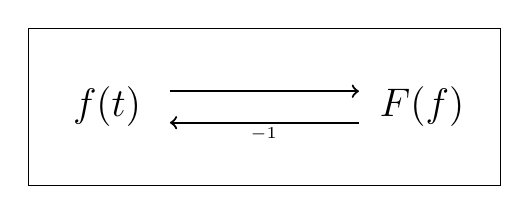
\begin{tikzpicture}
        % Box
        \node[draw, minimum width=6cm, minimum height=2cm] at (0,0) {};
        
        % Left side: Larger Time domain function
        \node at (-2, 0) {\Large $f(t)$};
        
        % Right side: Larger Frequency domain function
        \node at (2, 0) {\Large $F(f)$};
        
        % Fourier transform arrow, closer to center
        \draw[->, thick] (-1.2, 0.2) -- (1.2, 0.2);
        \node at (0, 0.4) {\small $\fourier$};
        
        % Inverse Fourier transform arrow, closer to center
        \draw[<-, thick] (-1.2, -0.2) -- (1.2, -0.2);
        \node at (0, -0.4) {\small $\fourier^{-1}$};
    \end{tikzpicture}
    \end{center}
    Con $f : \mathbb{R} \rightarrow \mathbb{C}$ e $F : \mathbb{R} \rightarrow \mathbb{C}$. Sebbene quasi sempre lo spettro di una
funzione f è complesso, quindi tridimensionale, possiamo raccontare \textbf{frequenze} e \textbf{ampiezze} tramite le funzioni:
\begin{itemize}
    \item \textbf{Spettro d'Ampiezza} $|F(f)| : \mathbb{R} \rightarrow \mathbb{R}$
    \item \textbf{Spettro di Fase} $\angle F(f) : \mathbb{R} \rightarrow \mathbb{R}$
\end{itemize} 

\end{minipage}

\subsubsection{Trasformate Notevoli}
\newcommand{\fCouple}{\overset{\fourier}{\longleftrightarrow}}
\newcommand{\fAnticouple}{\overset{\fourier^{-1}}{\longleftrightarrow}}
\paragraph{Rettangolo.}\lezione{Lezione 11}{4/11/2024} La trasformata sicuramente più importante è quella del rettangolo:

\begin{align*}
    S(f) &= \int_{-\infty}^{+\infty} \text{rect}(t)e^{-j2\pi ft} dt \\
         &= \int_{-\frac{1}{2}}^{\frac{1}{2}} e^{-j2\pi ft}dt =\\
         &= -\frac{1}{2j \pi f}\left(e^{j\pi f} - e^{-j\pi f}\right) = \\
         &= -\frac{1}{j \pi f}\left( \frac{e^{j\pi f} - e^{-j\pi f}}{2j}\right) = \\
         &= \frac{\cancel{j}}{ \pi f}\left( \frac{e^{j\pi f} - e^{-j\pi f}}{2\cancel{j}}\right) = \\
         &= \frac{1}{\pi f} \sin(\pi f) \tag{per eq di Eulero} =\\
         &= \text{sinc}(t)
\end{align*}

\paragraph{Delta di Dirac}
La trasformata di Fourier della Delta è molto particolare:
\begin{align*}
    S(f) &= \int_{-\infty}^{+\infty} \delta(t) e^{-j2\pi ft}dt =\\
         &= e^{-j2\pi f0} \tag{per il campionamento \eqref{prop: camp}} = 1\\
\end{align*}
Possiamo interpretare questo risultato dicendo che lo spettro della delta è costituita da infiniti seni di frequenze che 
vanno da $-\infty$ a $+\infty$ tutti di modulo unitario
\paragraph{Delta di Dirac Traslata}
Anche la trasformata della Delta Traslata di $t_0$ è interessante:
\begin{align*}
    S(f) &= \int_{-\infty}^{+\infty} \delta(t - t_0) e^{-j2\pi ft}dt =\\
         &= e^{-j2\pi f t_0} \tag{per il campionamento \eqref{prop: camp}}
\end{align*}

\subsection{Trasformata di Fourier di Segnali Reali}
Consideriamo $s(t) \in \mathbb{R}$, $\forall t \in \mathbb{R}$:
\begin{align*}
    S(f) &= \int_{-\infty}^{+\infty} s(t) e^{-j2 \pi f t} dt=\\
         &= \int_{-\infty}^{+\infty} f(t) \left[\cos(-j2 \pi f t) + j \sin(-j2 \pi f t)\right] dt\\
         &= \int_{-\infty}^{+\infty} f(t)\cos(-j2 \pi f t)dt + j \int_{-\infty}^{+\infty} f(t)\sin(-j2 \pi f t)dt =\\
         &= \underbrace{\int_{-\infty}^{+\infty} f(t)\cos(j2 \pi f t)dt}_{\in \mathbb{R}} - j \underbrace{\int_{-\infty}^{+\infty} f(t)\sin(-j2 \pi f t)dt}_{\in \mathbb{R}} =\\ \tag{per simmetrie}
         &= \mathbb{R}e\left[S(f)\right] -j\mathbb{I}m\left[S(f)\right] 
\end{align*}
\subsubsection{Proprietà Trasformata di Segnali Reali}
\paragraph{Simmetria Hermitiana.} Consideriamo ora $S(-f)$:
    \begin{align*}
        \mathbb{R}e[S(-f)] &= \int_{-\infty}^{+\infty} f(t)\cos(-j2 \pi f t)dt =\\
                           &= \int_{-\infty}^{+\infty} f(t)\cos(j2 \pi f t)dt = \mathbb{R}e[S(f)] \tag{simmetria pari}
    \end{align*}
    \begin{align*}
        \mathbb{I}m[S(-f)] &= \int_{-\infty}^{+\infty} f(t)\sin(-j2 \pi f t)dt =\\
                           &= -\int_{-\infty}^{+\infty} f(t)\sin(j2 \pi f t)dt = -\mathbb{I}m[S(f)] \tag{simmetria dispari}
    \end{align*}
Un'altra simmetria simile la possiamo notare per \textbf{modulo} e \textbf{fase} di $S(f)$:
\begin{itemize}
    \item $|S(f)| = |S(-f)|$
    \item $\angle S(f) = -\angle S(-f)$
\end{itemize}
Da ciò possiamo notare che la trasformata della frequenza opposta ha lo stesso modulo della trasformata di partenza ma fase opposta;
questa è proprio la definizione di \textbf{coniugato} e definisce la \textbf{Simmetria Hermitiana}:
\begin{equation}
    S(-f) = \overline{S(f)} \tag{se $s(t) \in \mathbb{R}$}
\end{equation}
Normalmente un grafico di un segnale si rappresenta in forma \textbf{bilatera}, considerando sia i tempi negativi sia positivi.
Da questi calcoli abbiamo dimostrato che la trasformata di un qualsiasi segnale reale è sempre simmetrico rispetto alle ordinate
per cui molto spesso la trasformata viene rappresentata in forma \textbf{monolatera}, cioè solo per $t > 0$.
\paragraph{Linearità.}
La trasformata di Fourier è un operatore lineare:
\begin{equation}
    \fourier\left[ax(t) + by(t)\right] = a\fourier\left[x(t)\right] + b\fourier\left[y(t)\right]
\end{equation}
\paragraph{Dimostrazione. }
\begin{align*}
    \fourier\left[ax(t) + by(t)\right] &= \int_{-\infty}^{+\infty} \left[ax(t) + by(t)\right] e^{-j2\pi ft}dt=\\
                                           &= \int_{-\infty}^{+\infty} ax(t)e^{-j2\pi ft} + by(t)e^{-j2\pi ft}dt= \\
                                           &= a\int_{-\infty}^{+\infty} x(t)e^{-j2\pi ft} + b\int_{-\infty}^{+\infty}y(t)e^{-j2\pi ft}dt=\\
                                           &= a\fourier\left[x(t)\right] + b\fourier\left[y(t)\right]
\end{align*}
\paragraph{Dualità.}
Dato un segnale $s(t)$ tale che $\fourier[s(t)] = S(f)$, allora:
\begin{equation}
    \fourier[S(t)] = s(-f)
\end{equation}
\paragraph{Dimostrazione.}
\begin{align*}
    \fourier[S(t)] &= \int_{-\infty}^{+\infty} S(t) e^{-j2\pi ft} dt =\\
                   &= \int_{-\infty}^{+\infty} S(t) e^{j2\pi (-f)t}dt = s(-f) 
\end{align*}
Ossia otteniamo la formula di sintesi.

\paragraph{Traslazione dei Tempi.}
Dato un segnale $s(t)$ tale che $\fourier[s(t)] = S(f)$, allora:
\begin{equation}\label{prop: traslTempi}
    \fourier[s(t - t_0)] = S(f)e^{-j2 \pi ft_0}
\end{equation}
\paragraph{Dimostrazione.}
Iniziamo a considerare:
\begin{equation*}
    \fourier[s(t - t_0)] = \int_{-\infty}^{+\infty} s(t - t_0) e^{-j2\pi ft} dt
\end{equation*}
Effettuiamo ora questo scambio di variabili $\begin{cases}
    t' = t - t_0\\
    dt' = dt
\end{cases}$
\begin{align*}
    &= \int_{-\infty}^{+\infty} s(t') e^{-j2\pi f(t' + t_0)} dt' =\\
    &= \int_{-\infty}^{+\infty} s(t') e^{-j2\pi ft'}\underbrace{e^{-j2\pi ft_0}}_{costante} dt' =\\
    &= e^{-j2\pi ft_0}\int_{-\infty}^{+\infty} s(t') e^{-j2\pi ft'} dt' =\\
    &= S(f)e^{-j2 \pi ft_0}
\end{align*}

\paragraph{Traslazione nelle Frequenze.}
Dato $\fourier[s(t - t_0)] = \int_{-\infty}^{+\infty} s(t - t_0) e^{-j2\pi ft} dt$ allora si dimostra per dualità che:
\begin{equation}
    \fourier[s(t)e^{-j2\pi ft_0}] = S(f + f_0)
\end{equation}

\paragraph{Modulazione d'Ampiezza}
Dato $S(f) = \fourier[s(t)]$ e il segnale modulato $s_m(t) = s(t) \cos(2\pi f_c t)$ allora
\begin{align*}
    \fourier\{s(t) \cos(2\pi f_ct)\} &=  \int_{-\infty}^{+\infty}s(t) \frac{e^{j2\pi f_ct}+e^{-j2\pi f_ct}}{2} dt=\\
                        &=  \int_{-\infty}^{+\infty}s(t) \frac{1}{2} (e^{j2\pi f_ct}+e^{-j2\pi f_ct}) dt=\\
                        &=  \int_{-\infty}^{+\infty}\frac{1}{2} (s(t)e^{j2\pi f_ct}+s(t)e^{-j2\pi f_ct}) dt=\\
                        &=  \frac{1}{2} (S(f + f_0) + S(f - f_0))
\end{align*}

\paragraph{Banda di un Segnale}
Data una coppia $s(t) \fCouple S(f)$ si definisce \textbf{Banda di un Segnale} $B$ il supporto delle frequenze,ossia
l'insieme delle frequenze per le quali il modulo non è nullo:
\begin{equation}
    B = \{f \in \mathbb{R} : |S(f)| \neq 0\}
\end{equation}

\paragraph{Bandwidth} 
La Bandwidth o \textbf{Larghezza di Banda} $BW$ rappresenta \textbf{l'estensione} di B, ossia:
\begin{equation}
    BW = f_2 - f_1
\end{equation}
Dove $f_2, f_1$ sono le frequenze estremità della Banda. 
NB: Dal momento che la trasformata di un segnale reale è, per la simmetria Hermitiana, simmetrica rispetto alle y,
allora la $BW$ viene definito sullo \textbf{Spettro Monolatero}. Possiamo definire una nuova classificazione dei segnali:
\paragraph{Segnali In Banda Base.}Sono segnali che contengono l'origine nella Banda.
\paragraph{Segnali In Banda Passante.}Sono segnali che non contengono l'origine nella Banda.
\section{Markov Decision Processes}
Tutti i problemi finora affrontati ricadevano sempre entro la famiglia dell\textbf{inferenza}. D'ora in poi tratteremo l'altro
ramo dell'IA, ossia l'\textbf{apprendimento}.
La prima classe di problemi che affronteremo in questo ambito sono i \textbf{Markov Decision Processes}.
\paragraph{Descrizione Generale.}
\begin{itemize}
    \item Gli agenti hanno come obiettivo il raggiungimento di uno \textbf{stato terminale} (può essere unico, multiplo o assente se l'agente dev'essere sempre attivo)
    \item L'ambiente è \textbf{Stocastico} e \textbf{Single-Agent}
    \item Esiste un \textbf{Orizzonte Temporale} entro cui agire
\end{itemize}
\paragraph{Formalizzazioni.}
\begin{itemize}
    \item \textbf{Insieme degli Stati}: $S : \{s_1, s_2, \dots\}$
    \item \textbf{Stato Iniziale}: $s_i \in S$
    \item \textbf{Stato Terminale}: $s_T \in S$
    \item \textbf{Azioni possibili per lo stato s}: $A(s)$
    \item \textbf{Modello di Transizione Stocastica}: dato $s \in S, a \in A(s), s' \in S$ con la transizione da $s$ a $s'$ con azione $a$,
    il modello di transizione $f$ indica la probabilità di finire proprio sullo stato s', ossia:
    \begin{equation}
        f(s,a,s') =  \mathbb{P}(s' | s,a)
    \end{equation} 
    \item \textbf{Reward}: ad ogni transizione l'agente riceve un reward (il corrispondente di costo negli algoritmi di search) che 
    dev'essere \textbf{additivo}
    \item \textbf{Orizzone H}: ossia le epoche di decisione per un MDP; oltre quest'epoca, tutto non viene più considerato. Se $H = \infty$ allora
    il processo termina se e solo se l'agente raggiunge uno stato terminale
\end{itemize}
\subsection{Markovianità}
Dato un processo stocastico che genera una \textbf{sequenza aleatoria} $s_1, s_2, \dots, s_n$ (aleatoria perchè l'ambiente è stocastico),
un processo si dice \textbf{Markoviano} se e solo se \textit{l'esito di un'azione dipende solo dallo stato corrente e non dagli stati precedenti}, ossia:
\begin{equation}
    \mathbb{P}(s_{t+1} | s_t,a_t,s_{t-1},a_{t-1},\dots, s_0, a_0) = \mathbb{P}(s_{t+1} | s_t,a_t)
\end{equation}
In parole povere, se un processo è markoviano, tutte le informazioni necessarie per potere scegliere la mossa migliore è già contenuta nello stato attuale stesso.
Assumere che un processo sia markoviano, inoltre permette di facilitare di molto i calcoli non perdendo di generalità (questo perchè la markovianità è un'assunzione realistica in molti contesti).

\subsection{Risoluzione di un MDP}
In un problema MDP, quello che si cerca è la \textbf{policy} $\pi$:
\begin{equation*}
    \pi : S \rightarrow A
\end{equation*}
Questa è una funzione \textbf{deterministica} che mappa ad ogni stato un'azione. Il nostro obiettivo è, una volta risolto il problema,
quello di rendere l'agente un \textbf{agente reflex} che sa già, ad ogni stato, le azioni da compiere. Naturalmente la difficoltà sta nel 
trovare una policy che \textbf{ottimizzi} un parametro (ad esempio il reward).

\subsection{Stimare la bontà di una policy}
Rispetto ai problemi precedenti, stimare la bontà di una strategia o un percorso risultava essere piuttosto intuitiva. Qui le cose si complicano 
per 2 motivi:
\begin{itemize}
    \item Le transizioni sono stocastiche, dunque i reward sono \textbf{incerti}
    \item Viene imposto un \textbf{orizzonte temporale }$h$
\end{itemize}
La \textbf{policy ottima} deve dunque \textbf{massimizzare il valore atteso della somma dei reward}.
\paragraph{Definizione}
\begin{itemize}
    \item Data una sequenza $s_1,\dots, s_n$ di stati generati da $\pi$
    \item Dati un reward associato ad ogni stato $R_1,R_2,\dots, R_n$
    \item Data $U(s_1,s_2,\dots,s_n) = R_1 + R_2 + \dots + R_n$
\end{itemize} 
La policy ottima $\pi^*$  deve generare il valore atteso della somma dei reward non peggiore di ogni altra policy:
\begin{equation}
    \pi^* = \arg \max_{\pi} \mathbb{E}_{\pi}\left[ U(s_0,s_1, \dots, s_n)\right]
\end{equation}
Possiamo dunque notare come i reward assegnati influenzino notevolmente la policy:
\begin{itemize}
    \item per $R < 0$, possiamo notare che la policy ottima induca l'agente a trovare lo stato terminale migliore nella maniera più efficiente
    \item per $R \ll 0$ possiamo notare che la policy ottima induca l'agente a trovare un qualsiasi stato terminale nel minor numero di passi possibili
    \item per $R > 0$ la policy ottima indurrà l'agente a non raggiungere mai lo stato terminale  
\end{itemize}
\newpage
\section{Filtri}
\subsection{Filtri Ideali}
\lezione{Lezione 13}{11/11/2024}
I filtri ideali sono filtri descritti matematicamente e con proprietà difficilmente replicabili con esattezza
tramite circuiti reali.\\
Consideriamo un \textbf{Sistema senza Distorsione} nella seguente forma:
\begin{equation}
    y(t) = Ax(t - t_0)
\end{equation}
La trasformata di questo sistema è la seguente:
\begin{equation}
    Y(f) = AX(f)e^{-j2\pi ft_0} \tag{proprietà \eqref{prop: traslTempi}}
\end{equation}
Con $H(f) = Ae^{-j2\pi ft_0} = \begin{cases}
    |H(f)| = A\\
    \angle H(f) = (-2\pi t_0) f 
\end{cases}$
\subsection{Filtri Lineari Ideali}
Definiamo \textbf{Filtro Lineare Ideale} un filtro nella seguente forma:
\begin{equation}
    H(f) = \begin{cases}
        Ae^{-j2\pi ft_0} & \text{ se } f \in B\\
        0 & \text{ se } f \not\in B
    \end{cases}
\end{equation}
Dove $B$ è detta \textbf{Banda Passante di Un filtro}, perchè non annulla la frequenza del segnale in ingresso.

\subsubsection{Filtro Passa-Basso (Ideale)}
Questo filtro fa passare tutte le frequenze al di sotto di una \textbf{Frequenza di Taglio} $f_T$, ossia:
\begin{equation}
    H(f) = \begin{cases}
        Ae^{-j2\pi ft_0} & \text{ se } |f| < f_T\\
        0 & \text{ altrimenti}
    \end{cases}
\end{equation}
Possiamo calcolare la sua \textbf{risposta all'impulso} (Considerando $A = 1, t_0 = 0$):
\begin{equation*}
    H_{LP} = \begin{cases}
        1 & \text{ se } |f| < f_T\\
        0 & \text{ altrimenti}
    \end{cases} = \text{rect}\left(\frac{t}{2f_T}\right)
\end{equation*}
\begin{equation*}
    \underbrace{\text{rect}\left(\frac{f}{2f_T}\right)}_{H(f)} \fAnticouple \underbrace{2f_T\text{sinc}(2f_Tt)}_{h(t)}
\end{equation*}

\subsubsection{Filtro Passa-Alto (Ideale)}
Questo filtro fa passare, al contrario, tutte le frequenze al di sopra di una \textbf{Frequenza di Taglio} $f_T$, ossia:
\begin{equation}
    H(f) = \begin{cases}
        Ae^{-j2\pi ft_0} & \text{ se } |f| \geq f_T\\
        0 & \text{ altrimenti}
    \end{cases}
\end{equation}
Possiamo calcolare la sua \textbf{risposta all'impulso} (Considerando $A = 1, t_0 = 0$):
\begin{equation*}
    H_{HP} = \begin{cases}
        1 & \text{ se } |f| \geq f_T\\
        0 & \text{ altrimenti}
    \end{cases} = 1 - \text{rect}\left(\frac{t}{2f_T}\right)
\end{equation*}
\begin{equation*}
    \underbrace{1 - \text{rect}\left(\frac{f}{2f_T}\right)}_{H(f)} \fAnticouple \underbrace{\delta(t) - 2f_T\text{sinc}(2f_Tt)}_{h(t)}
\end{equation*}

\subsubsection{Filtro Passa-Banda (Ideale)}
Questo filtro fa passare tutte le frequenze entro un intervallo $\left[f_m,f_M\right]$, ossia:
\begin{equation}
    H(f) = \begin{cases}
        Ae^{-j2\pi ft_0} & \text{ se } f_m < |f| < f_M\\
        0 & \text{ altrimenti}
    \end{cases}
\end{equation}
Possiamo calcolare la sua \textbf{risposta all'impulso} (Considerando $A = 1, t_0 = 0$):
\begin{equation*}
    H_{BP} = \begin{cases}
        1 & \text{ se } f_m < |f| < f_M\\
        0 & \text{ altrimenti}
    \end{cases} = \text{rect}\left(\frac{f - f_c}{B}\right) + \text{rect}\left(\frac{f + f_c}{B}\right)
\end{equation*}
\begin{equation*}
    \underbrace{\text{rect}\left(\frac{f - f_c}{B}\right) + \text{rect}\left(\frac{f + f_c}{B}\right)}_{H(f)} \fAnticouple \underbrace{2B\text{sinc}(Bt)\cos(2\pi f_ct)}_{h(t)}
\end{equation*}

\subsubsection{Filtro Arresta-Banda (Ideale)}
Questo filtro fa passare, al contrario, tutte le frequenze al di fuori di un intervallo $\left[f_m,f_M\right]$, ossia:
\begin{equation}
    H(f) = \begin{cases}
        Ae^{-j2\pi ft_0} & \text{ se } \leq f_m \textbf{ o } |f| \geq f_M \\
        0 & \text{ altrimenti}
    \end{cases}
\end{equation}
Possiamo calcolare la sua \textbf{risposta all'impulso} (Considerando $A = 1, t_0 = 0$):
\begin{equation*}
    H_{BS} = \begin{cases}
        1 & \text{ se } f_m < |f| < f_M\\
        0 & \text{ altrimenti}
    \end{cases} = 1 - \text{rect}\left(\frac{f - f_c}{B}\right) - \text{rect}\left(\frac{f + f_c}{B}\right)
\end{equation*}
\begin{equation*}
    \underbrace{1 - \text{rect}\left(\frac{f - f_c}{B}\right) - \text{rect}\left(\frac{f + f_c}{B}\right)}_{H(f)} \fAnticouple \underbrace{\delta(t) - 2B\text{sinc}(Bt)\cos(2\pi f_ct)}_{h(t)}
\end{equation*}

\subsection{Filtri Reali}
I filtri reali, sono invece, quelli costruiti tramite componenti circuitali. I circuiti analogici, per chiare limitazioni fisiche,
non potranno mai riprodurre fedelmente i comportamenti dei filtri ideali.
\subsubsection{Circuito RC}
Il circuito RC corrisponde ad un \textbf{Filtro Passa-Basso Reale} per il fatto che la risposta all'impulso assomiglia
a quella di un filtro passa-basso. In un circuito possiamo immaginare un impulso come una scarica di intensità infinita
che attraversa il circuito in un tempo infinitesimo e carica il condensatore instantaneamente di $1A$, e poi si scarica seguendo
un andamento \textbf{esponenziale decrescente} (circa). La risposta all'impulso possiamo descriverla cosi:
\begin{equation}
    h(t) = u(t)e^{-\frac{t}{RC}}
\end{equation}
Con $R$ la \textbf{resistenza del circuito} e $C$ la \textbf{capacità del condensatore}. $RC$ viene detto \textbf{tempo caratteristico} del sistema.
La trasformata di questa risposta all'impulso è la seguente:
\begin{equation*}
    H(f) = \frac{1}{1 + j2\pi f RC}
\end{equation*}
Se consideriamo la frequenza di taglio $f_T = \frac{1}{2\pi RC}$ abbiamo che:
\begin{equation}
    H(f) = \frac{1}{1 + j\frac{f}{f_T}}
\end{equation} 
Analizziamo modulo e frequenza di questa risposta in frequenza:
\begin{equation}
    |H(f)| = 
    \begin{cases}
        1 &\text{ se } f \ll f_T\\
        \frac{1}{\sqrt{2}} &\text{ se } f = f_T \\
        \ll 1 &\text{ se } f \gg f_T   
    \end{cases}
\end{equation}
\begin{equation}
    \angle H(f)= 
    \begin{cases}
        \approx 0 &\text{ se } f \ll f_T\\
        -\frac{\pi}{4} &\text{ se } f = f_T \\
        -\frac{\pi}{2} &\text{ se } f \gg f_T   
    \end{cases}
\end{equation}
Il grafico di risposta all'impulso dovrebbe essere:
\begin{center}
    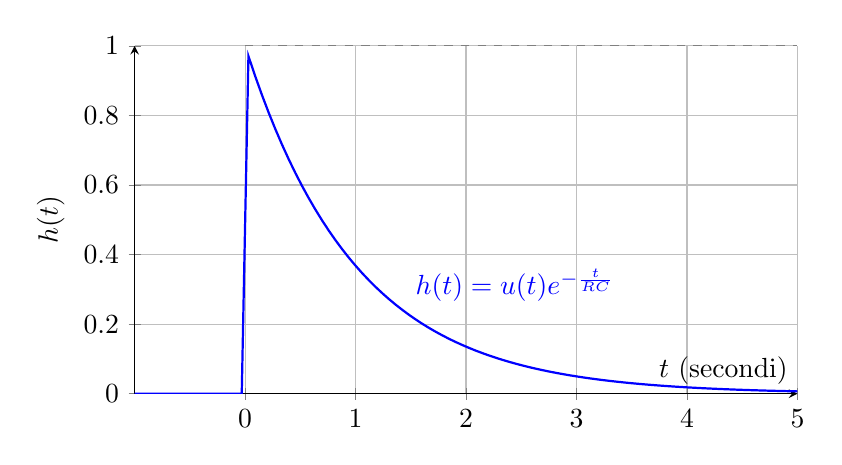
\begin{tikzpicture}
        \begin{axis}[
            width=10cm, height=6cm,
            xlabel={$t$ (secondi)},
            ylabel={$h(t)$},
            xmin=-1, xmax=5,
            ymin=0, ymax=1,
            xtick={-1,0,1,2,3,4,5},
            ytick={0,0.2,0.4,0.6,0.8,1},
            grid=both,
            domain=-1:5,
            samples=100,
            axis x line=middle, % Sposta l'asse x al centro
            axis y line=left, % Lascia l'asse y a sinistra
            legend pos=north east
        ]
        
        % Grafico della scarica del condensatore con condizione a zero per t<0
        \addplot[blue, thick] {x < 0 ? 0 : exp(-x)} node[pos=0.5, above right] {$h(t) = u(t)e^{-\frac{t}{RC}}$};
        
        % Linea per V0
        \addplot[dashed, gray] coordinates {(0,1) (5,1)};
        \node at (axis cs:0.2,1) [anchor=south west] {$V_0$};
    
        \end{axis}
    \end{tikzpicture}
\end{center}
Dal momento che per $f > f_T$ la risposta in frequenza decresce per $1/f$ ogni volta, questo filtro viene detto
\textbf{filtro del I ordine}. 
\paragraph{Ordine n-esimo di un Filtro.}Si definisce Ordine n-esimo di un Filtro, un filtro che decresce al di fuori
della banda di $1/f^n$ 
\newpage
\subsubsection{Approccio Value Iteration}
Questo primo approccio di risoluzione tramite programmazione dinamica dell MDP si basa sulla costruzione, iterazione dopo
iterazione, di una value function $V_k$ che convergerà a $V^*$:
\begin{itemize}
    \item per \textbf{k = 0}: $V_0(s) = 0$  $\forall s$
    \item per \textbf{k > 0}: $V_{k+1}(s) \leftarrow \max_{a}\underbrace{\sum_{s'} P(s'|s,a)[R(s,a,s') + \gamma V_k(s')]}_{Q(s,a)}$
\end{itemize}
Quell'ultima operazione viene detta \textbf{Bellman Update} e l'operatore $\rightarrow$ è detta \textbf{Operatore di Bellman}.
La risoluzione del problema avviene calcolando ad ogni iterazione la value function che \textbf{monotonicamente convergerà} a
$V^*$. Quindi, ad una certa iterazione, se $V_k$ soddisfa il \textbf{test di convergenza} allora abbiamo trovato la value function.\\

\tikzstyle{startstop} = [rectangle, rounded corners, minimum width=3cm, minimum height=1cm, text centered, draw=black, fill=red!30]
\tikzstyle{process} = [rectangle, minimum width=3cm, minimum height=1cm, text centered, draw=black, fill=blue!30]
\tikzstyle{decision} = [diamond, aspect=2, minimum width=2cm, minimum height=0.5cm, text centered, draw=black, fill=green!30]
\tikzstyle{arrow} = [thick,->,>=stealth]


\begin{center}
    \begin{tikzpicture}[node distance=2cm]

        % Nodes
        \node (start) [startstop] {$k \rightarrow 0$,  $V_0(s) = 0, \forall s$};
        \node (iterate) [process, below of=start] {
        \begin{minipage}{4cm}
            $k \leftarrow k + 1$\\
            $\forall a, s: \text{ Calcola }Q(s, a)$
        \end{minipage}};
        \node (update) [process, below of=iterate] {Aggiorna $V_k(s) = \max_a Q(s, a)$};
        \node (check) [decision, below of=update, yshift=-0.5cm] {Convergenza?};
        \node (end) [startstop, below of=check, yshift=-2cm] {$\pi(s) = \arg\max_a Q(s, a)$};
        %\node (repeat) [process, left of=check, xshift=-4cm] {Ripeti per il prossimo stato};%
        
        % Arrows
        \draw [arrow] (start) -- (iterate);
        \draw [arrow] (iterate) -- (update);
        \draw [arrow] (update) -- (check);
        \draw [arrow] (check.south) -- ++(0,-2) node[midway, right] {Sì} -- (end.north);
        \draw [arrow] (check.west) -- ++(-2,0) node[midway, above] {No} -- ++(0,4.5) -- (iterate.west);
        %\draw [arrow] (repeat.north) |- (iterate.west);
        
        \end{tikzpicture}
\end{center}

Il \textbf{Test di Convergenza} possiamo implementarlo come la condizione:
\begin{equation}
    |\max_s \{V_{k+1}(s) - V_k(s)\} - \min_s \{V_{k+1}(s) - V_k(s)\}| \leq \varepsilon
\end{equation}
Ossia \textit{lo span (differenza tra val massimo e minimo tra i $V_k$ di 2 iterazioni dev'essere meno di un epsilon)}, oppure:
\begin{equation}
    \sum_{s} |V_{k+1} (s) - V_k(s)| \leq \varepsilon
\end{equation} 
Ossia \textit{la somma delle differenze tra i value function tra 2 iterazioni dev'essere meno di epsilon}.
Sebbene quest'algoritmo sia efficace (dimostreremo dopo perchè), non sempre è efficiente, perchè $V_k$ potrebbe \textbf{convergere lentamente}.


\subsubsection{Dimostrazione di Convergenza}
Osservando l'operatore di Bellman:
\begin{equation}
    V_{k+1}(s) \leftarrow \max_{a} \sum_{s'} P(s'|s,a)[R(s,a,s') + \gamma V_k(s')]
\end{equation}
Possiamo accorgerci di una grande somiglianza con i \textbf{giochi stocastici} e, ancora meglio, con \textbf{Expectimax} (dal momento
che quell'algoritmo puntava a massimizzare il valore atteso del reward di ogni mossa). Possiamo ricondurre un MDP ad un \textbf{gioco
stocastico ad 1 giocatore MAX}. Quindi possiamo dire che calcolare $V_k(s)$ corrisponde a risolvere un gioco stocastico di livello $k$.
Tra l'albero di gioco a profondità $k$ e $k + 1$ possiamo visualizzare questa relazione:
\begin{center}
    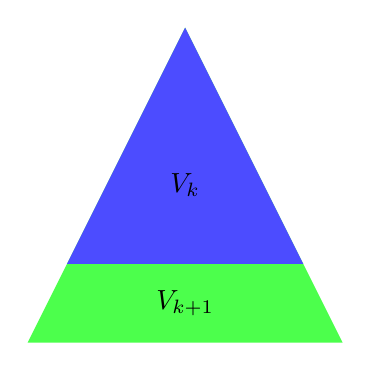
\begin{tikzpicture}

        % Triangolo verde (più grande)
        \fill[green!70] (0,0) -- (2,4) -- (4,0) -- cycle;
        
        % Triangolo blu (più piccolo e innestato)
        \fill[blue!70] (0.5,1) -- (2,4) -- (3.5,1) -- cycle;
        
        % Etichette (opzionale)
        \node at (2,2) {$V_k$};
        \node at (2,0.5) {$V_{k+1}$};
        
        \end{tikzpicture} 
\end{center}
Inoltre possiamo vedere l'albero $V_k$ come un albero di altezza $k + 1$ che ha nell'ultimo livello ($k+1$) i reward tutti nulli,
per cui $V_k$ e $V_{k+1}$ differiscono solo per i reward che all'ultimo livello sono (o potrebbero essere) $\neq 0$.\\
Sappiamo che un qualsiasi Reward $R$ è limitato:
\begin{equation*}
    R_{min} \leq R \leq R_{max}
\end{equation*}
Dunque i casi possibili sono 2:
\paragraph{Caso Migliore}Ogni reward $R = R_{max}$, per cui $V_{k+1}(s) = V_k(s) + \gamma^k R_{max}$
\paragraph{Caso Peggiore}Ogni reward $R = R_{min}$, per cui $V_{k+1}(s) = V_k(s) + \gamma^k R_{min}$
Allora un qualsiasi reward sarà sempre tra il caso migliore e il caso peggiore:
\begin{equation}
    V_k + \gamma^k R_{min} \leq V_{k+1} \leq V_k + \gamma^k R_{max}
\end{equation}
Ora facendo tendere $k \rightarrow +\infty$ otteniamo:
\begin{equation}
    V_k + 0 \leq V_{k+1} \leq V_k + 0
\end{equation}
Ossia, $V_k$ non cambia dunque abbiamo trovato una soluzione all'equazione di Bellman e che sarà necessariamente ottima.
\subsubsection{Policy Extraction}
\lezione{Lezione 15}{18/11/2024}
Una volta calcolata la value function, dovremmo semplicemente estrarre la policy a partire dai valori calcolati applicando la formula:
\begin{equation}
    \pi^* = \arg \max_a \sum_{s'} P(s' | s,a)[R(s,a,s') + \gamma V^*(s')]
\end{equation}
Possiamo però notare quanto sia inefficiente l'algoritmo per 2 grandi motivi:
\begin{itemize}
    \item Nel caso peggiore dovremmo considerare per ogni azione qualsiasi transizione ($O(|S|^2 \times |A|)$)
    \item Non è semplice trovare un $\varepsilon$ giusto per il test di convergenza
\end{itemize}
Possiamo tuttavia notare che, già dalle prime iterazioni, avevamo individuato la policy ottima, ancora prima della value function.
Per questo motivo possiamo cambiare totalmente approccio e iterare sulle policy.

\subsubsection{Policy Iteration}
Questo è un algoritmo che possiamo descrivere così:
\begin{itemize}
    \item Scelgo inizialmente una policy $\pi$ casuale
    \item \textbf{Policy Evaluation}: calcolo $V^\pi (s)$
    \item \textbf{Policy Extraction}: estraggo una nuova policy $\pi'$ a partire da $V^\pi (s)$
\end{itemize}
Nonappena succede che $\pi = \pi'$, ho trovato la policy ottima. Dal momento che itero sulla policy, $V^\pi(s)$ è :
\begin{equation}
    V^\pi(s) = Q(s,\pi(s)) = \sum_{s'} P(s' | s,a)[R(s,a,s') + \gamma V^*(s')]
\end{equation}
Non essendoci il $\max$, quella è un'equazione lineare. Mettendo a sistema le equazioni per ogni stato, otteniamo un sistema lineare
da risolvere.

\section{Reinforcement Learning}
Potrebbe capitare che l'agente che deve risolvere l'MDP$ = \left<P,R\right>$ (dove $P$ sono le probabilità di transizione e $R$ sono i reward)
senza conoscere P e R. In ambiente sconosciuto, dunque, l'agente non potrebbe applicare dynamic programming per risolvere il problema, o almeno all'inizio.
All'inizio, un agente può solo assumere che le azioni siano stocastiche e che esistano dei reward (deterministici). In queste
condizioni l'agente deve alternare fasi di \textbf{esplorazione}, in cui costruire una \textbf{stima del mondo} e questo può portare
l'agente a fare decisioni con reward molto bassi, perchè conoscere il mondo ha più valore, e fasi di \textbf{Exploitation} ossia di 
massimizzazione dei reward (che è il suo obiettivo principale).

\subsection{Passive Reinforcement Learning}
In questa prima fase, presenteremo una forma più semplice dell'RL, ossia \textbf{l'RL passivo}: un agente, in un ambiente sconosciuto,
conosce una policy $\pi$ e deve stimarne la \textit{bontà}, o meglio la \textbf{value function} $V^*$. A differenza dei casi precedenti,
qui non si conoscono nè $P(s'|s,a)$ nè $R(s',a,s)$ per cui dovremo stimare. Il problema di tali approcci è che dipendono troppo dall'esperienza,
per cui, con nessuna modalità di reasoning, tali agenti non sapranno rispondere ad un input se non l'hanno già incontrato in passato.

\subsubsection{Adaptive Dynamic Programming}
In questo primo approccio all Passive Reinforcement Learning, \textbf{Model Based}:
\begin{enumerate}
    \item Esploro il mondo usando la policy $\pi$ in un \textbf{episodio}, ossia una sequenza di mosse, e colleziono i reward e le probabilità in \textbf{dataset}
    \item Costruisco una \textbf{stima} di P e di R dal Modello Del Mondo che ho raccolto nel dataset, ossia:
    \begin{gather}
        \widehat{P}(s'|s,a) = \frac{\#(s,a,s')}{\#(s,a)} \\
        \widehat{R}(s,a,s') = R(s,a,s') 
    \end{gather}
    \item Calcolo della nuova policy ottima $\pi^*$ usando l'approccio dynamic programming sul modello stimato
\end{enumerate}

\subsubsection{Stima Diretta}
Un altro approccio usando la Passive RL \textbf{Model Free} è la \textbf{Stima Diretta}, ossia:
\begin{enumerate}
    \item Genero un dataset dall'esplorazione
    \item Per ogni stato $s$ misuro i reward accumulati per tutto l'episodio
    \item La stima sarà la \textbf{media aritmetica}:
    \begin{equation}
        \widehat{V}^\pi(s) = \frac{1}{k}\sum_{i = 1}^{k} \text{TotR}^s_i
    \end{equation}
    dove $\text{TotR}^s_i$ rappresenta il reward totale accumulato all'episodio $i$ partendo dallo stato $s$
\end{enumerate}
Il problema di questo approccio è che le stime vengono fatto facendo la (sbagliata) assunzione che gli stati siano indipendenti tra loro.
\subsubsection{Temporal Difference Learning}
\lezione{Lezione 16}{21/11/2024}
Questa tecnica \textbf{model-free} corregge i difetti della stima diretta, ossia dell'assunzione di indipendenza tra le transizioni
(che era ciò che rendeva non affidabile l'approccio). L'idea di base di quest'approccio è quello di calcolare, ad ogni transizione
una stima di $\widehat{V}^{\pi}(s)$ migliore.\\
Inizialmente, si parte da una stima per nulla buona, ossia che $\widehat{V}^{\pi}(s) = 0, \forall s$. Appena l'agente esegue
un azione $\pi(s)$ e transita da $s$ a $s'$ ottiene il reward $R(s,\pi(s),s')$, per cui, dopo aver acquisito una prima \textit{esperienza} di 
s. Definisco poi z nella seguente maniera:
\begin{equation}
    z = R(s,a,s') + \gamma \widehat{V}^{\pi}(s')
\end{equation} E corrisponde all'esperienza acquisita nell'ultima transizione. 
Aggiorno, allora, nella seguente maniera la state-function:
\begin{equation}
    \widehat{V}^{\pi}(s) \leftarrow \widehat{V}^{\pi}(s) + \alpha(z - \widehat{V}^{\pi}(s))
\end{equation}
Quest'operazione aggiorna $\widehat{V}^{\pi}(s)$ tramite una combinazione tra ciò che conosco già ($\widehat{V}^{\pi}(s)$) e
la \textbf{differenza temporale}, ossia la differenza tra ciò che ho scoperto nell'ultima iterazione ($z$) 
e quello che sapevo già ($\widehat{V}^{\pi}(s)$). La combinazione avviene attraverso un fattore $\alpha$, il \textbf{learning rate}.
Analizziamone i 2 possibili casi:
\begin{itemize}
    \item $\alpha = 1$: considero solo $z$, per cui l'agente non ricorda niente di ciò che ha appreso in precedenza
    \item $\alpha = 0$: l'agente è molto conservativo e qualsiasi nuova esperienza non cambia la sua state-function 
\end{itemize}
Possiamo riscrivere l'update nella seguente maniera, sostituendo $z$ con l'espressione precedente:
\begin{equation}
    \widehat{V}^{\pi}(s) \leftarrow (1- \alpha)\widehat{V}^{\pi}(s) + \alpha(R(s,a,s') + \gamma \widehat{V}^{\pi}(s'))
\end{equation}
In questa equazione, dunque, compare la dipendenza tra gli stati $s$ e $s'$ per cui viene corretto il problema principale della \textbf{stima diretta}.
Generalizziamo questo ragionamento: consideriamo ora $z_i = R(s,\pi(s),s') + \gamma \widehat{V}_{i - 1}^{\pi}(s')$ dove
$\widehat{V}_{i}^{\pi}(s)$ è la stima di $\widehat{V}^{\pi}(s)$ all'iterazione $i$. Al passo k-esimo possiamo riscrivere
l'equazione nella maniera seguente:
\begin{equation}
    \widehat{V}_k^{\pi}(s) = \alpha\sum_{i = 1}^{k} \left[\underbrace{(1- \alpha)^{k - i}z_{k - i}}_{\text{temporal differences}}+ (1 - \alpha)^k \underbrace{\widehat{V}_0^{\pi}(s')}_{\text{bootstrap}}\right]
\end{equation}
La cosa interessante di questo approccio è che la \textbf{stima iniziale} o \textbf{bootstrap}, viene man mano corretta e andrà a contare sempre di meno nella stima finale.
Solitamente viene inizializzata a 0. Il \textbf{temporal difference} viene invece calcolato tramite \textbf{media mobile esponenziale} in modo che 
le esperienze più recenti sono più rilevanti mentre quelle più passate di meno.

\paragraph{Convergenza della Temporal Difference Learning.}
Il learning rate che avevamo introdotto per combinare esperienza e conoscenza non è altro che un coefficiente per bilanciare
\textbf{exploitation} e \textbf{exploration} che avevamo incontrato in UCB per risolvere il MAB Problem. Affinchè $\widehat{V}^{\pi}(s)$ 
converga al vero $V(s)$ è necessario che $\alpha$ vari. Solitamente $\alpha $ varia in funzione del numero di volte $N_s$ che è
stato visitato un nodo $s$, per cui possiamo esprimerlo come funzione $\alpha(N_s)$. Si può dimostrare che, affinchè converga,
$\alpha(N_s)$ deve presentare le seguenti proprietà:
\begin{equation}
    \sum_{n = 1}^{\infty} \alpha(n) = \infty
\end{equation}
 \begin{equation}
    \sum_{n = 1}^{\infty} \alpha^2(n) < \infty
\end{equation}
Solitamente si adotta, per $\alpha$, una funzione che cresce con $O(\frac{1}{n})$

\subsubsection{Potenza Del Disturbo}
Una volta individuata la forma e l'entità del disturbo, possiamo calcolare la potenza di questo segnale:
\begin{equation*}
    P_Q = \int_{-\infty}^{+\infty} e^2 f_{eq}(e)de
\end{equation*}
Abbiamo visto prima che, se gli intervalli $\Delta$ sono sufficientemente piccoli, possiamo assumere che $f_{eq}(e)$ sia una
funzione di densità di probabilità uniforme, che ha questa forma:
\begin{equation}
    f_{eq}(e) = \begin{cases}
        \frac{1}{\Delta} &\text{ se } -\frac{1}{\Delta} \leq e \leq \frac{1}{\Delta}\\
        0                &\text{ altrimenti}
    \end{cases}
\end{equation}
Allora possiamo riscrivere l'equazione precedente:
\begin{align*}
    P_Q &= \int_{-\frac{\Delta}{2}}^{+\frac{\Delta}{2}} \frac{1}{\Delta} e^2 de =\\
        &= \frac{1}{\Delta} \int_{-\frac{\Delta}{2}}^{+\frac{\Delta}{2}} e^2 de =\\
        &= \frac{1}{\Delta} \left( \frac{\Delta^3}{24} +  \frac{\Delta^3}{24}\right) =\\
        &= \frac{\Delta^2}{12}
\end{align*}
Quello che abbiamo trovato è la \textbf{Potenza Media dell'errore di Quantizzazione}. 

\paragraph{Signal Noise Ratio.}La potenza Media dell'errore, tuttavia,
ci dice ben poco poichè tale valore dev'essere sempre confrontato con la potenza del segnale disturbato,
per questo motivo ha più senso parlare del rapporto, anche detto \textbf{SIgnal Noise Ratio (SNR)}:
\begin{equation}
    \text{SNR} = \frac{P_\text{signal}}{P_\text{noise}}
\end{equation}
I possibili $P_\text{signal}$ che possiamo scegliere per calcolare quel rapporto sono la \textbf{Potenza di Picco} o la \textbf{Potenza Media}

\paragraph{Potenza Di Picco.}Sappiamo che il valore $x$ del segnale da quantizzare è sempre limitato, ossia:
\begin{equation*}
    V_{MIN} \leq x < V_{MAX}
\end{equation*}
Dove $\{V_{MIN}; V_{MAX}\}$ è detta \textbf{Escursione del Segnale}. Considereremo, per semplicità, \textbf{segnali bipolari}
ossia segnali in cui vale che $V_{MIN} = - V_{MAX}$. Possiamo esprimere questi 2 valori in termini di \textbf{Escursione Picco-Picco} $V_{pp}$:
\begin{gather}
    V_{pp} = V_{MAX} - V_{MIN}\\
    V_{MAX} = \frac{V_{pp}}{2}\\
    V_{MIN} = -\frac{V_{pp}}{2}\\
\end{gather}
Grazie a ciò, possiamo calcolarci la \textbf{potenza di picco} del segnale:
\begin{equation}
    P_{s,\text{picco}} = \left(\frac{V_{pp}}{2}\right)^2 = \frac{V^2_{pp}}{4}
\end{equation}
Sappiamo inoltre che per come abbiamo introdotto la quantizzazione, vale che:
\begin{equation*}
    \Delta = \frac{V_{pp}}{M} = \frac{V_{pp}}{2^n} \Rightarrow V_{pp} = 2^n\Delta
\end{equation*}
Allora possiamo scrivere il \textbf{Signal Noise Ratio di Picco}:
\begin{align*}
    SNR_{Q,\text{Peak}} &= \frac{\frac{V^2_{pp}}{4}}{\frac{\Delta^2}{12}} =\\
                        &= \frac{\frac{\Delta^2 2^{2n}}{4}}{\frac{\Delta^2}{12}}=\\
                        &= 3 \cdot 2^{2n}
\end{align*}
\paragraph{Potenza Media.}Oltre alla potenza di picco, possiamo esprimere la potenza del segnale in termini di \textbf{potenza media del segnale}:
\begin{equation}
    P_{s,\text{Media}} = f_{Picco} \cdot P_{s,\text{picco}}
\end{equation}
Dove $f_{Picco}$ è detto \textbf{fattore di picco}. Inoltre $0 \leq f_{Picco} \leq 1$.
Grazie a ciò possiamo esprimere il \textbf{Signal Noise Ratio Medio}:
\begin{align*}
    SNR_{Q,\text{Medio}} &= f_{Picco} \cdot \frac{P_{s,\text{picco}}}{P_Q} =\\
                         &= f_{Picco} \cdot SNR_{Q,\text{Peak}} =\\
                         &=  f_{Picco} \cdot 3 \cdot 2^{2n}
\end{align*}
Riconducendo dunque il rapporto di potenza segnale rumore in funzione dei \textbf{bit di campionamento} possiamo intuire che più
saranno i bit di campionamento, più il disturbo sarà minore, per questo motivo $n$ è anche detta \textbf{Risoluzione di Quantizzazione}. Inoltre, ogni bit in più di quantizzazione migliora il rapporto di un fattore 4.

\subsubsection{Decibel}
In generale, quando in fisica si ha a che fare con rapporto di potenze, ha più senso il confronto su scala logaritmica, per cui possiamo
definire i \textbf{decibel} sia in riferimento alle ampiezze, sia in riferimento alle potenze.
\begin{gather}
    dB_A = 20 \lg_{10} \frac{A_1}{A_2} \\
    dB_P = 10 \lg_{10} \frac{P_1}{P_2} 
\end{gather}
Le 2 formule sono state scelte in modo tale che il decibel per le ampiezze e per le potenze siano \textbf{invarianti} (parlare dell'una o dell'altra non fa differenza).

\paragraph{SNR in Decibel}
\begin{align*}
    dB(SBR_{Q,P}) &= 10 \lg_{10} \frac{P_{s,p}}{P_Q}=\\
                  &= 10 \lg_{10} 3 \cdot 2^{2n} =\\
                  &= 4,77 + 6,02n
\end{align*}
\begin{align*}
    dB(SBR_{Q,Media}) = dB(f_{picco}) + 4,77 + 6,02n
\end{align*}
Importante osservare che $dB(f_{picco}) < 0$ dal momento che $0 \leq f_{picco} \leq 1$ 

\newcommand{\DFT}{\xrightarrow{\text{DFT}}}
\newcommand{\IDFT}{\xrightarrow{\text{DFT}^{-1}}}
\newcommand{\DTFT}{\xrightarrow{\text{DTFT}}}

\subsection{Discrete Time Fourier Transform (DTFT)}
Per mostrare il teorema di nyquist, eravamo riusciti, già in precedenza \eqref{eq: sampleSpectre}, a calcolare la trasformata di Fourier
di un segnale campionato. Il limite di quella trasformata è che lo spettro del segnale campionato $S_C(f)$ continuava ad essere
legato, in qualche modo, allo spettro del segnale di partenza $S(f)$. Per cui, è necessario un altro strumento che permetta di
calcolare lo spettro di un segnale \textbf{tempo-discreto} $s(nT_S) \approx x(n)$ dove $n \in \mathbb{Z}$, in funzione dei campioni.\\
Partendo dal segnale campionato $s_c(t) = \sum_{n = -\infty}^{+\infty} s(nT_S)\delta(t - nT_S)$ la \textbf{trasformata discreta} sarà:
\begin{align*}
    S_C(f) &= \int_{-\infty}^{+\infty}s_c(t)e^{-j2\pi ft}dt =\\
           &= \int_{-\infty}^{+\infty} \sum_{n = -\infty}^{+\infty} s(nT_S)\delta(t - nT_S) e^{-j2\pi ft}dt=\\
           &= \sum_{n = -\infty}^{+\infty} s(nT_S) \int_{-\infty}^{+\infty} \delta(t - nT_S) e^{-j2\pi ft}dt
\end{align*}
Possiamo dire che $\delta(t - nT_S) e^{-j2\pi ft}$ è non nulla solo per $t = nT_S$.
A questo punto, scriviamo la \textbf{formula di Analisi della DTFT}:
\begin{equation}
    S_C(f) = \sum_{n = -\infty}^{+\infty} s(nT_S) e^{-j2\pi fnT_S}
\end{equation}
\paragraph{Spettro Periodico}Un'importante proprietà di questo spettro è che è periodico di periodo $f_s = \frac{1}{T_S}$. Dimostriamolo:
\begin{align*}
    S_C(f + kf_s) &= \sum_{n = -\infty}^{+\infty} s(nT_S) e^{-j2\pi (f + kf_s)nT_S} = \\
                  &= \sum_{n = -\infty}^{+\infty} s(nT_S) e^{-j2\pi fnT_S}  \underbrace{e^{-j2\pi kf_s nT_S}}_{e^{-j2\pi} = 1} =\\
                  &= \sum_{n = -\infty}^{+\infty} s(nT_S) e^{-j2\pi fnT_S} =\\
                  &= S_C(f)
\end{align*}

\subsection{DTFT Normalizzata}
Una volta effettuato il campionamento, sarebbe comodo pure dimenticarci il periodo di campionamento ed esprimere lo spettro in forma normalizzata,
ossia le cui frequenze anzichè andare da $0$ a $f_S$ vanno da $0$ a $1$. Per fare ciò dovremo effettuare un cambio di variabile:
\begin{equation*}
    x(t' = n) = s(t = nT_S)
\end{equation*}
Dove $t' = \frac{t}{T_S}$. Allora la \textbf{formula di analisi normalizzata} sarà:
\begin{align*}
    x(t' = n) \fCouple X(f') = S_C(f' = fT_S) =  \sum_{n = -\infty}^{+\infty} s(nT_S) e^{-j2\pi f'n}
\end{align*}
Solitamente $f' = \frac{f}{f_s}$, che è un numero puro, viene rappresentato come $0 \leq \phi \leq 1$, per cui:
\begin{equation*}
    x(n) \fCouple X(\phi)
\end{equation*}
Analogamente allo sviluppo in serie, possiamo individuare la \textit{"formula inversa"}, la \textbf{formula di Sintesi}:
\begin{equation}
    x(n) = \frac{1}{T_\phi} \int_{0}^{1} X(\phi)e^{+j2\pi \phi n}d\phi
\end{equation}

\subsubsection{Proprietà della DTFT}
\paragraph{Traslazione nei Tempi.}Data una coppia $x(n) \fCouple X(\phi)$ allora:
\begin{equation}
    x(n - m) \fCouple X(\phi)e^{-j2\pi \phi m}
\end{equation}
\paragraph{Traslazione nelle Frequenze.}Data una coppia $x(n) \fCouple X(\phi)$ allora:
\begin{equation}
    x(n)^{j2\pi \phi n} \fCouple X(\phi - \phi_0)
\end{equation}
\paragraph{Convoluzione.}Date le coppie $x(n) \fCouple X(\phi)$ e $y(n) \fCouple Y(\phi)$ allora:
\begin{equation}
    x(n) \ast y(n) \fCouple X(\phi)Y(\phi)
\end{equation}
Quindi, grazie alla DTFT, siamo riusciti a rappresentare un segnale campionato come una \textbf{combinazione lineare di seni}.

\subsection{Risoluzione e Durata di Campionamento}
Dato un segnale $s(n)$ rappresentato da $N$ campioni, campionato a frequenza $f_s = \frac{1}{T_s}$, nei \textbf{tempi} la \textbf{risoluzione di campionamento} è la frequenza di campionamento $f_s$.
Definiamo nei \textbf{tempi} \textbf{durata} $N \cdot T_S$, ossia il numero di campioni per il periodo di campionamento.\\
Nellle \textbf{frequenze} la \textbf{risoluzione} è $\Delta f = \frac{1}{NT_S}$, mentre la \textbf{durata}, nelle \textbf{frequenze}, corrisponde all'inverso del periodo. Per questo motivo,
se vogliamo aumentare la risoluzione delle frequenze, dobbiamo ascoltare il segnale per più tempo.

\subsection{Discrete Fourier Transform (DFT)}
Dunque, grazie al campionamento/quantizzazione e alla DTFT normalizzata, siamo riusciti a tradurre un segnale in una sequenza di valori,
ognuno dei quali rappresenta l'ampiezza del segnale per il campione $n$-esimo. Tuttavia, per la totale elaborazione di un segnale digitale, ciò non basta:
$X(\phi)$ continua infatti ad essere una funzione \textbf{continua}, ma noi, per rappresentare in un calcolatore ciò avremmo bisogno di un segnale che sia \textbf{discreto e periodico}
in modo da poterlo raccontare solo con un numero finito di campioni che costituisce un periodo (tanto tutti gli altri infiniti campioni si ripetono).\\
Abbiamo dimostrato già che la $X(\phi)$ sia \textbf{periodica}, manca solo la \textbf{discretezza}.\\
Finora abbiamo osservato che la trasformata di un segnale continuo e periodico, è un segnale discreto (vedi lo sviluppo in serie); mentre la trasformata di un segnale discreto  genera un segnale
continuo e periodico (vedi la DTFT). Per questo motivo, se noi trasformiamo un segnale discreto e periodico dovremo ottenere uno spettro ancora discreto e periodico:\\
Solitamente un segnale elaborato digitalmente ha una \textbf{durata finita} (dal momento che l'elaboratore ha memoria finita), per cui sarà campionato con un numero $N$ di campioni. 
Consideriamo ora la versione \textbf{periodicizzata} di $x(n)$ con periodo $N$, la funzione che alla fine si ripete fino all'infinito, ossia la funzione tale che:
\begin{equation}
    x(n) = x(n + iN) \text{  } \forall i \in \mathbb{Z}
\end{equation}
Analizziamo lo spettro di questo segnale \textbf{discreto e periodico}:
\begin{itemize}
    \item Dal momento che è \textbf{discreto}, tramite \textbf{DTFT} otteniamo uno spettro che è \textbf{periodico} (di periodo $f_s$ o $1$ nel caso sia normalizzato)
    \item Dal momento che è \textbf{periodico}, tramite \textbf{Sviluppo in serie} otteniamo uno spettro che è \textbf{discreto}, ossia una combinazione lineare di fasori di coefficiente $c_k$ di frequenza $\frac{k}{T}$ (ossia la k-esima armonica),ossia:
    \begin{equation*}
        x(n) = \sum_{k = -\infty}^{+\infty} c_k e^{-j2\pi \frac{k}{T}t} dt
    \end{equation*}
    Dove $c_k = \frac{1}{T}\int_{T} x(t)e^{-j2\pi \frac{k}{T}t}dt$. Dal momento che abbiamo discretizzato il periodo $T$ in $N$ campioni,
    possiamo riscrivere $c_k$ come:
    \begin{equation*}
        c_k = \frac{1}{N} \sum_{n = 0}^{N - 1} x(n) e^{-j2\pi \frac{k}{N}n}
    \end{equation*}
    L'espressione $\sum_{n = 0}^{N - 1} x(n) e^{-j2\pi \frac{k}{N}n}$ ricorda molto $X\left(\phi_k = \frac{k}{N}\right)$, per cui:
    \begin{equation*}
        c_k = \frac{1}{N} X(k)
    \end{equation*}
    Dove k definisce la k-esima frequenza di $\phi$, dal momento che $k = 0, 1, \dots, N-1$
\end{itemize}
In definitiva, possiamo enunciare le formule di \textbf{Discrete Fourier Transform (DFT)}:
\paragraph{Analisi:}
\begin{equation}
    x(n) \DFT X(k) = \sum_{n = 0}^{N - 1}x(n)e^{-j2\pi \frac{kn}{N}}
\end{equation}
\paragraph{sintesi:}
\begin{equation}
    X(k) \IDFT x(n) = \sum_{k = 0}^{N - 1}X(k)e^{j2\pi \frac{kn}{N}}
\end{equation}
Siamo dunque riusciti a trasformare anche la $X(k)$ in una sequenza numerica.



\subsubsection{Forma Matriciale della DFT}
Una forma alternativa (e forse computazionalmente più adatta) della DFT è in forma \textbf{matriciale}:
Dato $X(k) = \frac{1}{N} \sum_{n = 0}^{N - 1} x(n)e^{-j2\pi \frac{nk}{N}}$ possiamo vedere $X(k)$ e $x(n)$ come vettori, mentre $e^{-j2\pi \frac{nk}{N}}$ come una matrice $W$ e il tutto come un prodotto matriciale tra matrice e vettore:
\begin{equation}
    \begin{bmatrix}
        X(0) \\
        \vdots \\
        X(N-1)
        \end{bmatrix} = 
    \begin{bmatrix}
        & & & \\
        & W_{ij} = e^{-j2\pi \frac{ij}{N}} & \\
        & & &
        \end{bmatrix}
    \begin{bmatrix}
x(0) \\
\vdots \\
x(N-1)
\end{bmatrix}
\quad
\end{equation}
Ossia:
\begin{equation*}
    \overline{X} = W \overline{x}
\end{equation*}
Calcolare un prodotto del genere ha complessità computazionale $O(N^2)$. Tuttavia, è stato scoperto un modo più agevole e furbo
per tale calcolo, tramite la FFT (Fast Fourier Transform) che ha complessità computazionale $O(N \log N)$

\subsubsection{Proprietà della DFT}
\paragraph{Traslazione ciclica nei Tempi.}Data la coppia $x(n) \DFT X(k)$ allora:
\begin{equation}
    x(\left< n - a\right>_{N}) \DFT X(k)e^{j2\pi \frac{n}{N}k}
\end{equation}

\paragraph{Traslazione ciclica nelle Frequenze.}Data la coppia $x(n) \DFT X(k)$ allora:
\begin{equation}
    x(n)e^{j2\pi\frac{h}{N}n} \DFT X(\left< k - h\right>_{N})
\end{equation}

\paragraph{Convoluzione Ciclica.}Date la coppie $x(n) \DFT X(k)$ e $y(n) \DFT Y(k)$ allora:
\begin{equation}
    x(n) \circledast y(n) \DFT X(k)Y(k)
\end{equation}
\section{Machine Learning}
\subsection{Supervised Learning}
\lezione{Lezione 19}{9/12/2024}
La tecnica di \textbf{Supervised learning} è una delle principali in ML e si basa su un \textbf{Dataset di Training} $\tau = \langle(x_1,z_1),\dots,(x_n,z_n)\rangle$
dove $x_i$ è un vettore di lunghezza $m$ e rappresenta \textbf{l'input} e $z_i$ è uno scalare e rappresenta \textbf{l'output}. Tutti gli input $x_i$ hanno la stessa lunghezza.
Il dataset $\tau$ si ottiene a partire da un \textbf{processo} che è ignoto (gli input/output potrebbero essere umani o generati
da un algoritmo) che noi possiamo vedere come una funzione $f : \mathbb{R}^n \to \mathbb{R}$ tale che $x_i = f(x_i)$ che vogliamo scoprire.
Dal dataset di training la macchina deve trovare una $h(x)$ che approssima $f(x)$. Quindi l'apprendimento è \textit{supervisionato}
poichè la macchina apprende da degli esempi forniti da un arbitro/processo di cui ci fidiamo. In teoria, vorremmo che dopo l'addestramento
la macchina sappia rispondere correttamente a tutti gli $x_\text{NEW}$, detti \textbf{testcase}, non appartenenti al dataset.\\
Una cosa su cui soffermarsi è proprio la funzione $h$: è detta cosi perchè è una \textbf{ipotesi}, ossia tale funzione deve appartenere ad una
famiglia di funzioni scelta, per ipotesi, dall'esperto di ML. Funzioni più complesse permetteranno di imitare meglio la $f$ e di fare analisi
più interessanti, ma sono difficili da computare. Funzioni più semplici permetteranno invece di fare analisi più semplici ma anche di computarle in
meno tempo. Le classi di funzioni possono essere:
\begin{itemize}
    \item Lineari
    \item Polinomiali
    \item Sinusoidali
    \item Esponenziali
    \item Altre molto più complesse (di solito usate nei modelli di oggi)
\end{itemize}

\paragraph{Classe Lineare.}Per semplicità, studieremo il caso di funzioni lineari, che possiamo scrivere cosi:
\begin{equation}
    z = \theta[1,x]^T = 1\cdot\theta_0 + x_1\theta_1 + \dots x_n\theta_n
\end{equation}
Dove $\theta$ è un vettore riga di coefficienti, e $[1,x]^T$ è il vettore colonna che ha nel primo valore 1. Il compito Dunque
degli algoritmi di ML è di trovare il $\theta$ che permetta di \textbf{fittare} il modello sui dati. L'algoritmo che fa ciò è la
\textbf{Regressione Lineare Multivariata}

\subsubsection{Regressione Lineare Multivariata.}Quest'algoritmo effettua la regressione basandosi sul concetto di \textbf{loss}:
il loss è la distanza tra $f(x_i) = z_i$ e $h(x_i)$.
La funzione di loss più usata è lo \textbf{scarto quadratico medio}:
\begin{equation}
    (z_i - h(x_i))^2
\end{equation}
Per diversi motivi:
\begin{itemize}
    \item Lo scarto quadratico è \textbf{facile }da trattare matematicamente
    \item Amplifica i grandi errori e diminuisce i piccoli errori.
\end{itemize}
In particolare, quello che dev'essere minimizzato è il valore atteso di $\theta$, ossia: 
\begin{equation}
    \mathbb{E}[\theta] = \frac{1}{N} \sum_{i = 1}^{N}(z_i - h(x_i))^2
\end{equation}
Possiamo dunque dire che $h(x)$ è una funzione $h : \mathbb{R}^{n + 1} \to \mathbb{R}$, dal momento che $h$ deve anche stimare il $\theta_0$.
Per minimizzare il valore atteso possiamo scegliere 2 strade:
\paragraph{Approccio Analitico.}A partire dall'espressione della funzione di loss, dobbiamo calcolare la derivata prima. Una volta trovata dobbiamo
trovare la $x$ che annulli la derivata in un \textbf{punto di minimo globale}. Si potrebbe infatti ricadere nel caso di un punto di massimo o minimo locale,
che a noi non interessa.

\paragraph{Approccio Numerico.}Si calcola \textbf{iterativamente} il \textbf{gradiente} della funzione nel punto. Dal momento che il gradiente
è un vettore che indica sempre la \textbf{direzione di salita} dovremmo seguire il vettore opposto con un passo iterativo che noi definiamo così:\\
Dal momento che (considerando come funzione di loss lo scarto quadratico), calcoliamo così la i-esima derivata parziale:
\begin{equation}
        \frac{\partial \mathbb{E}[\theta]}{\partial \theta_i} = \frac{1}{2} \frac{\partial(z_i - h(x_i)^2)}{\partial \theta_i} = -(z_i - h(x_i))x_i 
\end{equation}
A questo punto, ad ogni iterazione effettuiamo l'aggiornamento di $\theta_i$:
\begin{equation}
    \theta_i \leftarrow \theta_i + \alpha\underbrace{(z_i - h(x_i))x_i}_{\text{correzione}}
\end{equation}
L'algoritmo che abbiamo visto viene detto \textbf{discesa del gradiente} perchè consiste appunto nel discendere dal gradiente della funzione.
Il fatto è che non possiamo calcolare tutto questo per ogni dato del dataset, piuttosto si scelgono alcuni esempi detti \textbf{minibatch}.
La ricerca dell'ottimo nell'intervallo può essere fatta pure tramite algoritmo di search \textbf{Hill Climbing}.
\subsubsection{Analisi Di Sistemi Discreti}
Consideriamo il sistema discreto $S[\cdot]$ t.c. $y(n) = S[x(n)] = x(n) \ast h(n)$ dove
\begin{equation*}
    y(n) = \sum_{i = -\infty}^{+\infty} h(i) x(n - i)
\end{equation*}
Dal momento che considereremo sistemi solo causali, la sommatoria diventa:
\begin{equation*}
    y(n) = \sum_{i = 0}^{+ \infty} h(i) x(n-i)
\end{equation*}
Per il calcolo della convoluzione noi possiamo considerare 2 grandi casi:
\begin{itemize}
    \item Risposta All'Impulso Finita (FIR)
    \item Risposta All'Impulso Infinita (IIR)
\end{itemize}

\paragraph{Risposta All'Impulso Finita}
In questo caso, il sistema non solo è causale ma la risposta all'impulso ha una durata \textbf{finita}, che noi possiamo scrivere come:
\begin{equation*}
    h(n) = \{h(0), h(1), \dots, h(D)\}
\end{equation*}
Dove $D$ è la durata. Grazie a ciò la convoluzione possiamo calcolarla come:
\begin{equation}
    \sum_{i = 0}^{D} h(i)x(n - i)
\end{equation}
Che noi possiamo calcolare campione per campione. Possiamo dunque vedere l'uscita come \textbf{combinazione lineare} tra ingresso attuale ($h(0)x(n)$)
e gli ingressi passati $h(1)x(n - 1), \dots, h(n)x(0)$. Questa è la formulazione in forma di \textbf{equazione alle differenze} di un filtro FIR.
Nel Dominio Z, dal momento che la risposta all'impulso è discreta, possiamo calcolarne la trasformata come combinazione lineare di trasformate di impulsi traslati, ossia:
\begin{equation}
    h(n) \zTransform H(z) = \sum_{i = 0}^{D} h(i)z^{-i}
\end{equation}
Conoscendo sia $X(z)$ che $H(z)$ posso conoscere facilmente $Y(z)$ e dunque $y(n)$ antritrasformando. Ciò permette di fare elaborazioni sia nel dominio
delle frequenze che nel dominio dei tempi.

\paragraph{Risposta All'Impulso Infinita}
In questo caso, la risposta all'impulso ha durata infinita, per cui non è possibile \textit{troncare} la serie e avere somme finite di termini.
Dobbiamo trovare degli escamotage per riscrivere la serie sottoforma di equazione recursiva.\\
Consideriamo l'integratore discreto che ha risposta all'impulso $h(n) = u(n)$ per cui il segnale in uscita del sistema è:
\begin{equation*}
    y(n) = \sum_{i = 0}^{+\infty}x(n - i)
\end{equation*}
Possiamo riscriverlo come:
\begin{align*}
    y(n) &= x(n) + \sum_{i = 0}^{+\infty}x(n - i -1) =\\
         &= x(n) + y(n - 1)
\end{align*}
Conoscendo $y(0)$ cioè all'istante iniziale, la computazione del segnale in uscita da questo sistema diventa davvero banale, ossia:
\begin{equation}
    y(n) = \begin{cases}
        y(0)    &\text{ se } n = 0\\
        x(n) + y(n - 1) &\text{ se } n > 0\\
    \end{cases}
\end{equation}
Consideriamo ora la risposta all'impulso $h(n) = a^n u(n)$, nel dominio Z la sua trasformata sarà $H(z) = \frac{1}{1 - az^{-1}}$. Nel dominio Z
quindi, la trasformata è rappresentabile da una formula in forma chiusa, ossia, dal momento che $Y(z) = X(z)H(z)$, allora:
\begin{align*}
    X(z) &= \frac{Y(z)}{H(z)} =\\
         &= Y(z) - \underbrace{az^{-1}Y(z)}_{\text{ritardo di 1}}
\end{align*}
Possiamo riscrivere il tutto come:
\begin{equation}
    y(n) = x(n) + ay(n-1)
\end{equation}
Allora, in generale, se abbiamo una $H(z)$ in forma razionale:
\begin{equation*}
    H(z) = \frac{N(z)}{D(z)}
\end{equation*}
$N(z)$ è la parte \textbf{FIR} che lega gli $y(n)$ agli \textbf{input passati}. $D(z)$ invece è la parte \textbf{IIR}, che lega l'uscita attuale alle uscite passate.
Per questo motivo, se $H(z)$ è in forma razionale possiamo ricavare molto facilmente le equazioni recursive che descrivono l'output di un sistema.\\
Più in genrale:
\begin{align*}
    H(z) = \frac{\sum_{i = 0}^{M}b_iz^{-i}}{\sum_{i = 0}^{N}a_iz_{-i}} = \frac{\sum_{i = 0}^{M}b_iz^{-i}}{1 - \sum_{i = 1}^{N}a_iz_{-i}}
\end{align*}
Inoltre, visto che $H(z) = \frac{Y(z)}{X(z)}$ eguagliando entrambi i membri otteniamo:
\begin{align*}
    Y(z)\left[1 - \sum_{i = 1}^{N} a_iz^{-i}\right] &= X(z)\left[\sum_{i = 0}^{M} b_iz^{-i}\right] =\\
    Y(z) &= Y(z)\sum_{i = 1}^{N} a_iz^{-i} + X(z)\sum_{i = 0}^{M}b_iz^{-i}=\\
    Y(z) &= \sum_{i = 0}^{N} a_iy(n - i) + \sum_{i = 0}^{M} b_ix(n - i)
\end{align*}
Questa equazione appena ottenuta che descrive l'output di un sistema discreto viene detta \textbf{equazione alle differenze in forma recursiva di un IIR}.
\subsection{Stabilità dei Filtri FIR}
Consideriamo un filtro generico con risposta all'impulso finita, ossia $h(n) = \{h(0),h(1),\dots,h(n)\}$. Sappiamo che per la proprietà di convoluzione
della trasformata Z $Y(z) = H(z)X(z) = \sum_{i = 0}^{M}h(i)z^{-i}X(z)$, allora possiamo riscrivere $H(z)$ come:
\begin{equation*}
    H(z) = \frac{Y(z)}{X(z)} = \frac{\sum_{i = 0}^{M}h(i)z^{-i}\cancel{X(z)}}{\cancel{X(z)}} = \sum_{i = 0}^{M}h(i)z^{-i}
\end{equation*}
Dunque $H(z)$ è un polinomio di grado $M$ e in $\mathbb{C}$ ha esattamente $M$ radici. Riscriviamo allora $H(z)$ in forma fattorizzata:
\begin{align*}
    H(z) &= h(0)(1 - z_1z^{-1})(1 - z_2z^{-1})\dots(1 - z_nz^{-1}) =\\
         &= h(0)\prod_{i = 1}^{M}(1 - z_iz^{-1})
\end{align*}
Avevamo già detto che un filtro digitale è stabile se e solo se tutti i poli sono contenuti nella circonferenza unitaria. Dal momento che 
la funzione di trasferimento di un filtro FIR non ha poli, allora i FIR sono \textbf{intrinsecamente stabili} a prescindere da quale sia la funzione
di trasferimento.

\subsection{Stabilità dei Filtri IIR}
Consideriamo ora un filtro con risposta all'impulso infinita nella sua forma recursiva:
\begin{align*}
    y(n) &= \sum_{i = 1}^{N}a_iy(n - i) + \sum_{i = 0}^{M}b_ix(n - i) =\\
    y(n) - \sum_{i = 1}^{N}a_iy(n - i) &= \sum_{i = 0}^{M}b_ix(n - i)
\end{align*}
Nel \textbf{dominio Z} tutto ciò diventa:
\begin{align*}
    Y(z)\left[ 1 - \sum_{i = 1}^{N}a_iz^{-i}\right] &= X(z)\left[\sum_{i = 0}^{M} b_iz^{-i}\right] \\
    \frac{Y(z)}{X(z)} &= \frac{\sum_{i = 0}^{M} b_iz^{-i}}{1 - \sum_{i = 1}^{N}a_iz^{-i}}\\
    H(z) &=  \frac{\sum_{i = 0}^{M} b_iz^{-i}}{1 - \sum_{i = 1}^{N}a_iz^{-i}}
\end{align*}
Da questa forma della funzione di trasferimento, possiamo notare che ha N poli e M zeri; riscriviamo il tutto come:
\begin{equation}
    H(z) = b_0 \frac{\prod_{i = 1}^{M}(1 - z_iz^{-i})}{\prod_{i = 1}^{(1 - p_iz^{-1})}}
\end{equation}
In questo caso, un filtro IIR è stabile se e solo se $\forall i |p_i| < 1$


\subsection{Sintesi di Filtri Digitali}
In questo campo esistono molte tecniche diverse di sintesi di filtri; una delle più famose e importanti consiste nel \textit{tradurre} l'equazione
alle differenze del sistema nel filtro HW vero e proprio. Per la realizzazione di un filtro digitale sono necessari alcuni componenti base:
\paragraph{Convertitore Analogico-Digitale}
Come abbiamo visto, per poter trattare un segnale digitale dobbiamo prima \textbf{campionarlo} e \textbf{quantizzarlo}. Questa funzione viene svolta 
da un elemento ADC che possiamo rappresentare cosi:
\begin{center}
    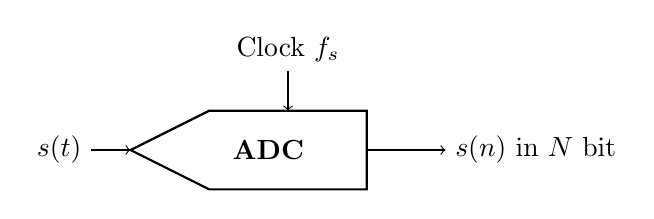
\begin{tikzpicture}[node distance=2cm, auto]

        % ADC shape: rectangle with triangular left side
        \draw[thick] (0, 0.5) -- (-1, 0) -- (0, -0.5) -- (2, -0.5) -- (2, 0.5) -- (0, 0.5) -- cycle;
        \node at (0.75, 0) {\textbf{ADC}};
        % Input signal (arrow pointing to the triangle)
        \node[left] at (-1.5, 0) {$s(t)$};
        \draw[->] (-1.5, 0) -- (-1, 0);
        
        % Clock signal (arrow pointing down to the ADC)
        \node[above] at (1, 1) {Clock $f_s$};
        \draw[->] (1, 1) -- (1, 0.5);
        
        % Output (N-bit quantization)
        \node[right] at (3, 0) {$s(n)$ in $N$ bit};
        \draw[->, draw, strike out] (2, 0) -- (3, 0);
        
        \end{tikzpicture}
\end{center}

\paragraph{Ritardatore}
Il ritardatore è un elemento che ritarda di 1 clock un campione. VIene realizzato come un vero e proprio registro, ossia
una batteria di flip-flop che al clock fanno passare in uscita i bit in entrata. Noi lo rappresentiamo come:
\begin{center}
    \begin{tikzpicture}[node distance=2cm, auto]

        % Rectangle with z^{-1} inside
        \node[draw, rectangle, minimum width=1cm, minimum height=1cm] (block) {\( z^{-1} \)};
        
        % Input x(n)
        \node[left of=block, node distance=3cm] (input) {\( x(n) \)};
        \draw[->, thick] (input) -- (block.west);
        
        % Output x(n-1)
        \node[right of=block, node distance=3cm] (output) {\( x(n-1) \)};
        \draw[->, thick] (block.east) -- (output);
        
        % Clock signal
        \node[above of=block, node distance=1.5cm] (clock) {Clock \( f_s \)};
        \draw[->, thick] (clock) -- (block.north);
        
        \end{tikzpicture}
\end{center}
Un ritardatore viene anche chiamato $z^{-1}$ poichè nel dominio Z:
\begin{equation}
    x(n - 1) \zTransform X(z)z^{-1}
\end{equation}

\paragraph{Moltiplicazione}
Un moltiplicatore a $n$ bit moltiplica gli n bit del segnale in ingresso con una costante e in uscita ha n bit. Viene rappresentato così:
\begin{center}
    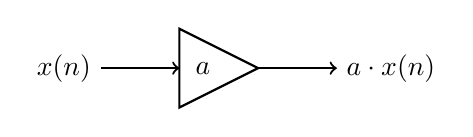
\begin{tikzpicture}[node distance=2cm, auto]

        % Triangle pointing right
        \draw[thick] (1,0) -- (0,0.5) -- (0,-0.5) -- cycle;
        
        % Label inside the triangle
        \node at (0.3, 0) {\( a \)};
        
        % Input x(n)
        \node[left] at (-1,0) {\( x(n) \)};
        \draw[->, thick] (-1,0) -- (0,0);
        
        % Output a*x(n)
        \node[right] at (2,0) {\( a \cdot x(n) \)};
        \draw[->, thick] (1,0) -- (2,0);
        
        \end{tikzpicture}
\end{center}

\paragraph{Sommatore}
Un sommatore somma i segnali in ingresso bit a bit, come un sommatore presente nelle ALU della CPU:
\begin{center}
    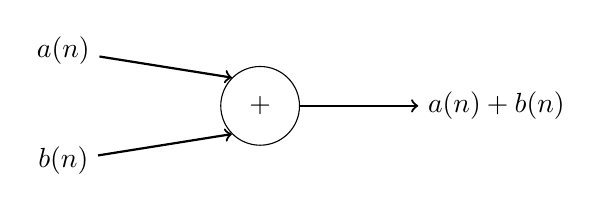
\begin{tikzpicture}[node distance=2cm, auto]

        % Circle with +
        \node[draw, circle, minimum size=1cm] (sum) {\( + \)};
        
        % Input a(n)
        \node[left of=sum, yshift=0.7cm, node distance=2.5cm] (inputA) {\( a(n) \)};
        \draw[->, thick] (inputA) -- (sum.135);
        
        % Input b(n)
        \node[left of=sum, yshift=-0.7cm, node distance=2.5cm] (inputB) {\( b(n) \)};
        \draw[->, thick] (inputB) -- (sum.225);
        
        % Output a(n) + b(n)
        \node[right of=sum, node distance=3cm] (output) {\( a(n) + b(n) \)};
        \draw[->, thick] (sum) -- (output);
        
        \end{tikzpicture}
\end{center}

\paragraph{Esempi di filtri digitali} Alcuni esempi di filtri digitali studiati sono i filtri a pettine (una sorta di filtro passa-basso reale) e i filtri notch (un filtro arresta-banda reale).

\subsection{Filtri a Pettine}
I filtri a pettine sono una famiglia di filtri che hanno la seguente funzione di trasferimento:
\begin{equation}
    H(z) = \frac{1 - z^{-M}}{1 - z^{-1}}
\end{equation}
Dove $M$ è l'\textbf{ordine del filtro}. Scriviamo l'equazione recursiva:
\begin{align*}
    H(z) &= \frac{Y(z)}{X(z)} = \frac{1}{M} \left(\frac{1 - z^{-M}}{1 - z^{-1}}\right)\\
         Y(z) &= \frac{1}{M}X(z)\left(\frac{1 - z^{-M}}{1 - z^{-1}}\right) =\\
         Y(z) &= \frac{1}{M}\left(X(z) - X(z)z^{-M} + Y(z)z^{-1}\right) 
\end{align*}
Antritrasformando otteniamo:
\begin{equation}
    y(n) = \frac{1}{M}\left(y(n-1) + x(n) - x(n - M)\right)
\end{equation}
Dove la $\frac{1}{M} $serve per normalizzare. Possiamo apprendere dalla funzione di trasferimento ha M zeri e 1 polo.
Applicando un polo laddove c'è uno zero, possiamo annullare l'effetto dello zero e non annullare la frequenza in 0.
L'utilità di questo filtro è che è un modesto filtro passa-basso, perchè ha la seguente risposta in frequenza:\\
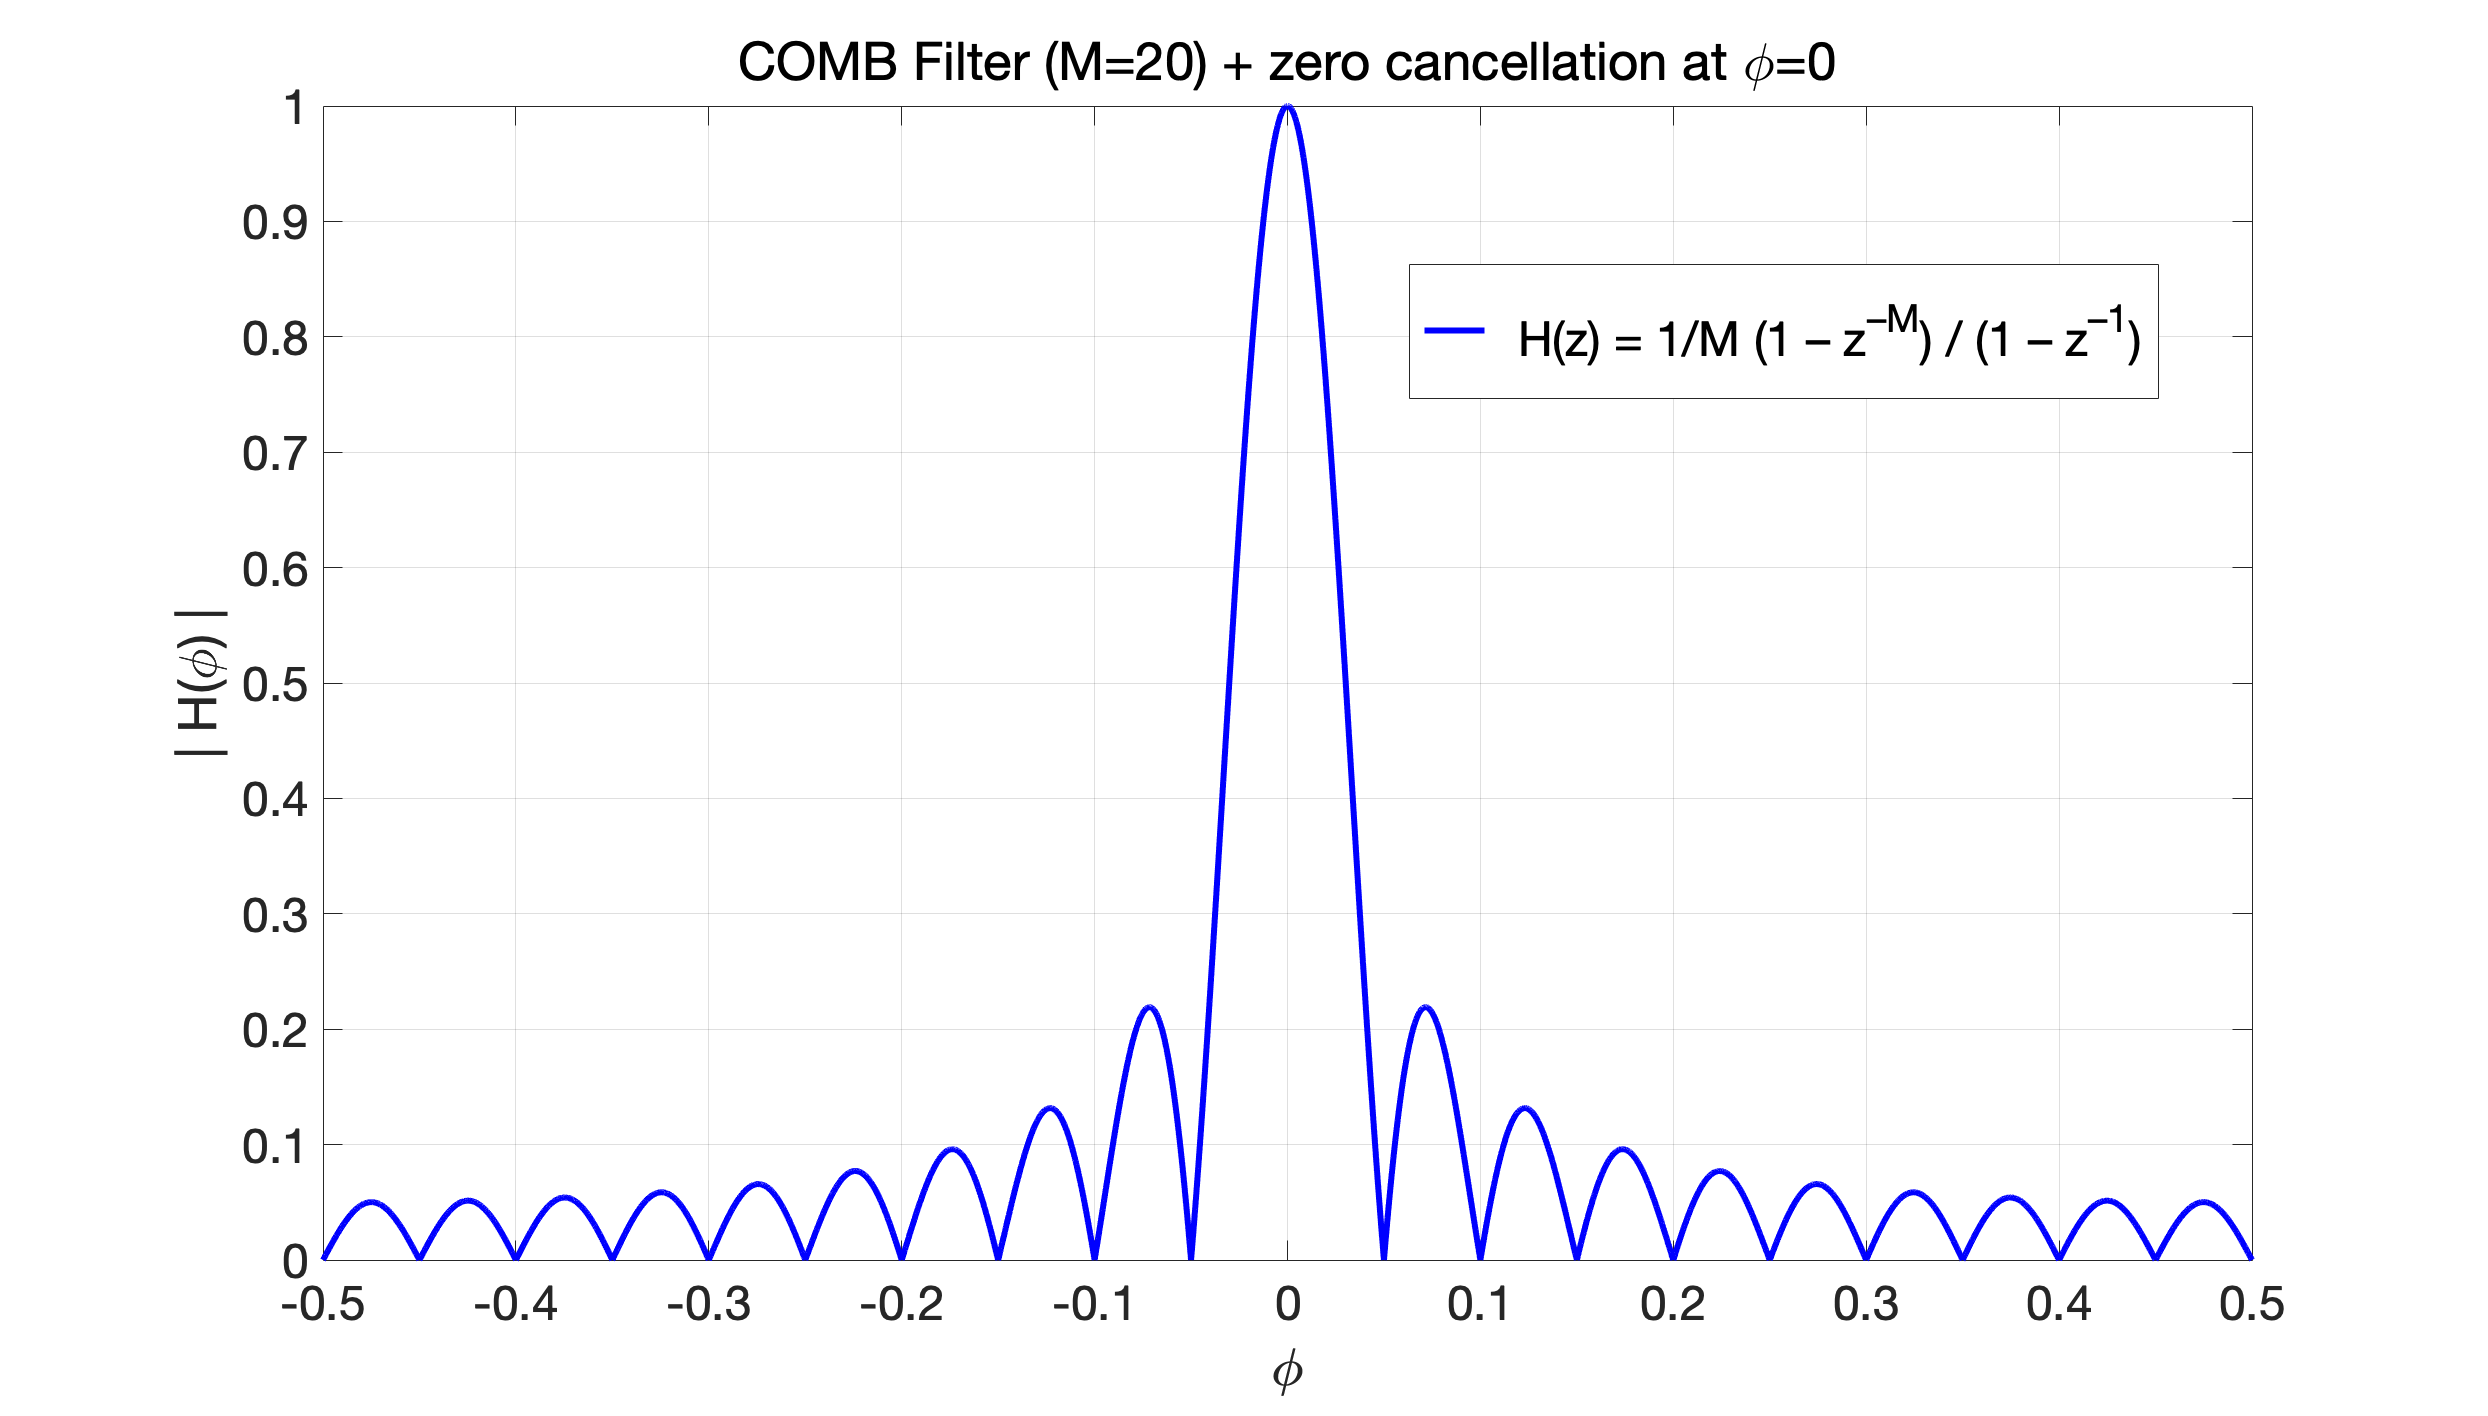
\includegraphics[width=15cm]{src/Comb20Filter.png}
Il lobo centrale fa passare tutto, mentre i lobi laterali attenuano sempre di più. Chiaramente le prestazioni
di questi filtri non sono così alte. Nota Bene: in teoria il filtro appena creato è instabile, poichè un polo
giace sulla circonferenza unitaria; nella stragrande maggioranza degli input il filtro risponde bene, sebbene
il problema si possa verificare con alcuni segnali (come il gradino unitario).

\subsection{Filtri Notch}
I filtri Notch sono filtri digitali arresta-banda, cioè che annullano particolari frequenze. Per farlo dobbiamo 
imporre uno zero sulla frequenza da eliminare. Dal momento che per i segnali reali vale la simmetria hermitiana
dobbiamo annullare anche il coniugato della frequenza da eliminare. Imponendo solo gli zeri, tuttavia, \textit{abbassiamo}
anche le frequenze vicine. Per cui dobbiamo imporre un polo molto vicino allo zero, con la stessa fase ma dentro il cerchio
unitario, in modo da renderlo stabile. Da tutto ciò otteniamo la seguente funzione di trasferimento:
\begin{equation}
    H(z) = \frac{(1 - z_Nz^{-1})(1 - \overline{z_N}z^{-1})}{(1 - p_Nz^{-1})(1 - \overline{p_N}z^{-1})}
\end{equation}
Dove $p_N = \alpha z_n$ con $0 \leq \alpha < 1$. Cerchiamo ora di estrapolarci l'equazione alle differenze:
\begin{align*}
    H(z) &= \frac{(1 - z_Nz^{-1})(1 - \overline{z_N}z^{-1})}{(1 - \alpha z_nz^{-1})(1 - \overline{\alpha z_n}z^{-1})} =\\
         &= \frac{1 - (z_N + \overline{z_N})z^{-1} + z_N\overline{z_N}z^{-2}}{1 - \alpha(z_N + \overline{z_N})z^{-1} + \alpha^2z_N\overline{z_N}z^{-2}} =\\
\end{align*}
Sappiamo, dalle proprietà dei numeri complessi che $z_N + \overline{z_N} = \mathbb{R}e[z]$ e che $z_N\overline{z_N} = \| z\| = 1 $ allora:
\begin{align*}
    H(z) &= \frac{1 - 2\mathbb{R}e[z_N]z^{-1} + z^{-2}}{1 - 2\alpha\mathbb{R}e[z_N]z^{-1} + \alpha^2z^{-2}}
\end{align*}
Sappiamo inoltre che $\mathbb{R}e[z_N] = \cos(2\pi\phi_N)$, allora:
\begin{align*}
    H(z) &= \frac{1 - 2\cos(2\pi\phi_N)z^{-1} + z^{-2}}{1 - 2\alpha\cos(2\pi\phi_N)z^{-1} + \alpha^2z^{-2}}
\end{align*}
Possiamo ricavarci dunque l'equazione alle differenze:
\begin{equation}
    y(n) = \alpha(2\cos(2\pi\phi_N))y(n-1) - \alpha^2y(n - 2) + x(n) - 4\cos(2\pi\phi_N)x(n-1) + x(n-2)
\end{equation}
La risposta in frequenza di questo filtro è la seguente, e possiamo notare come sia molto performante:\\
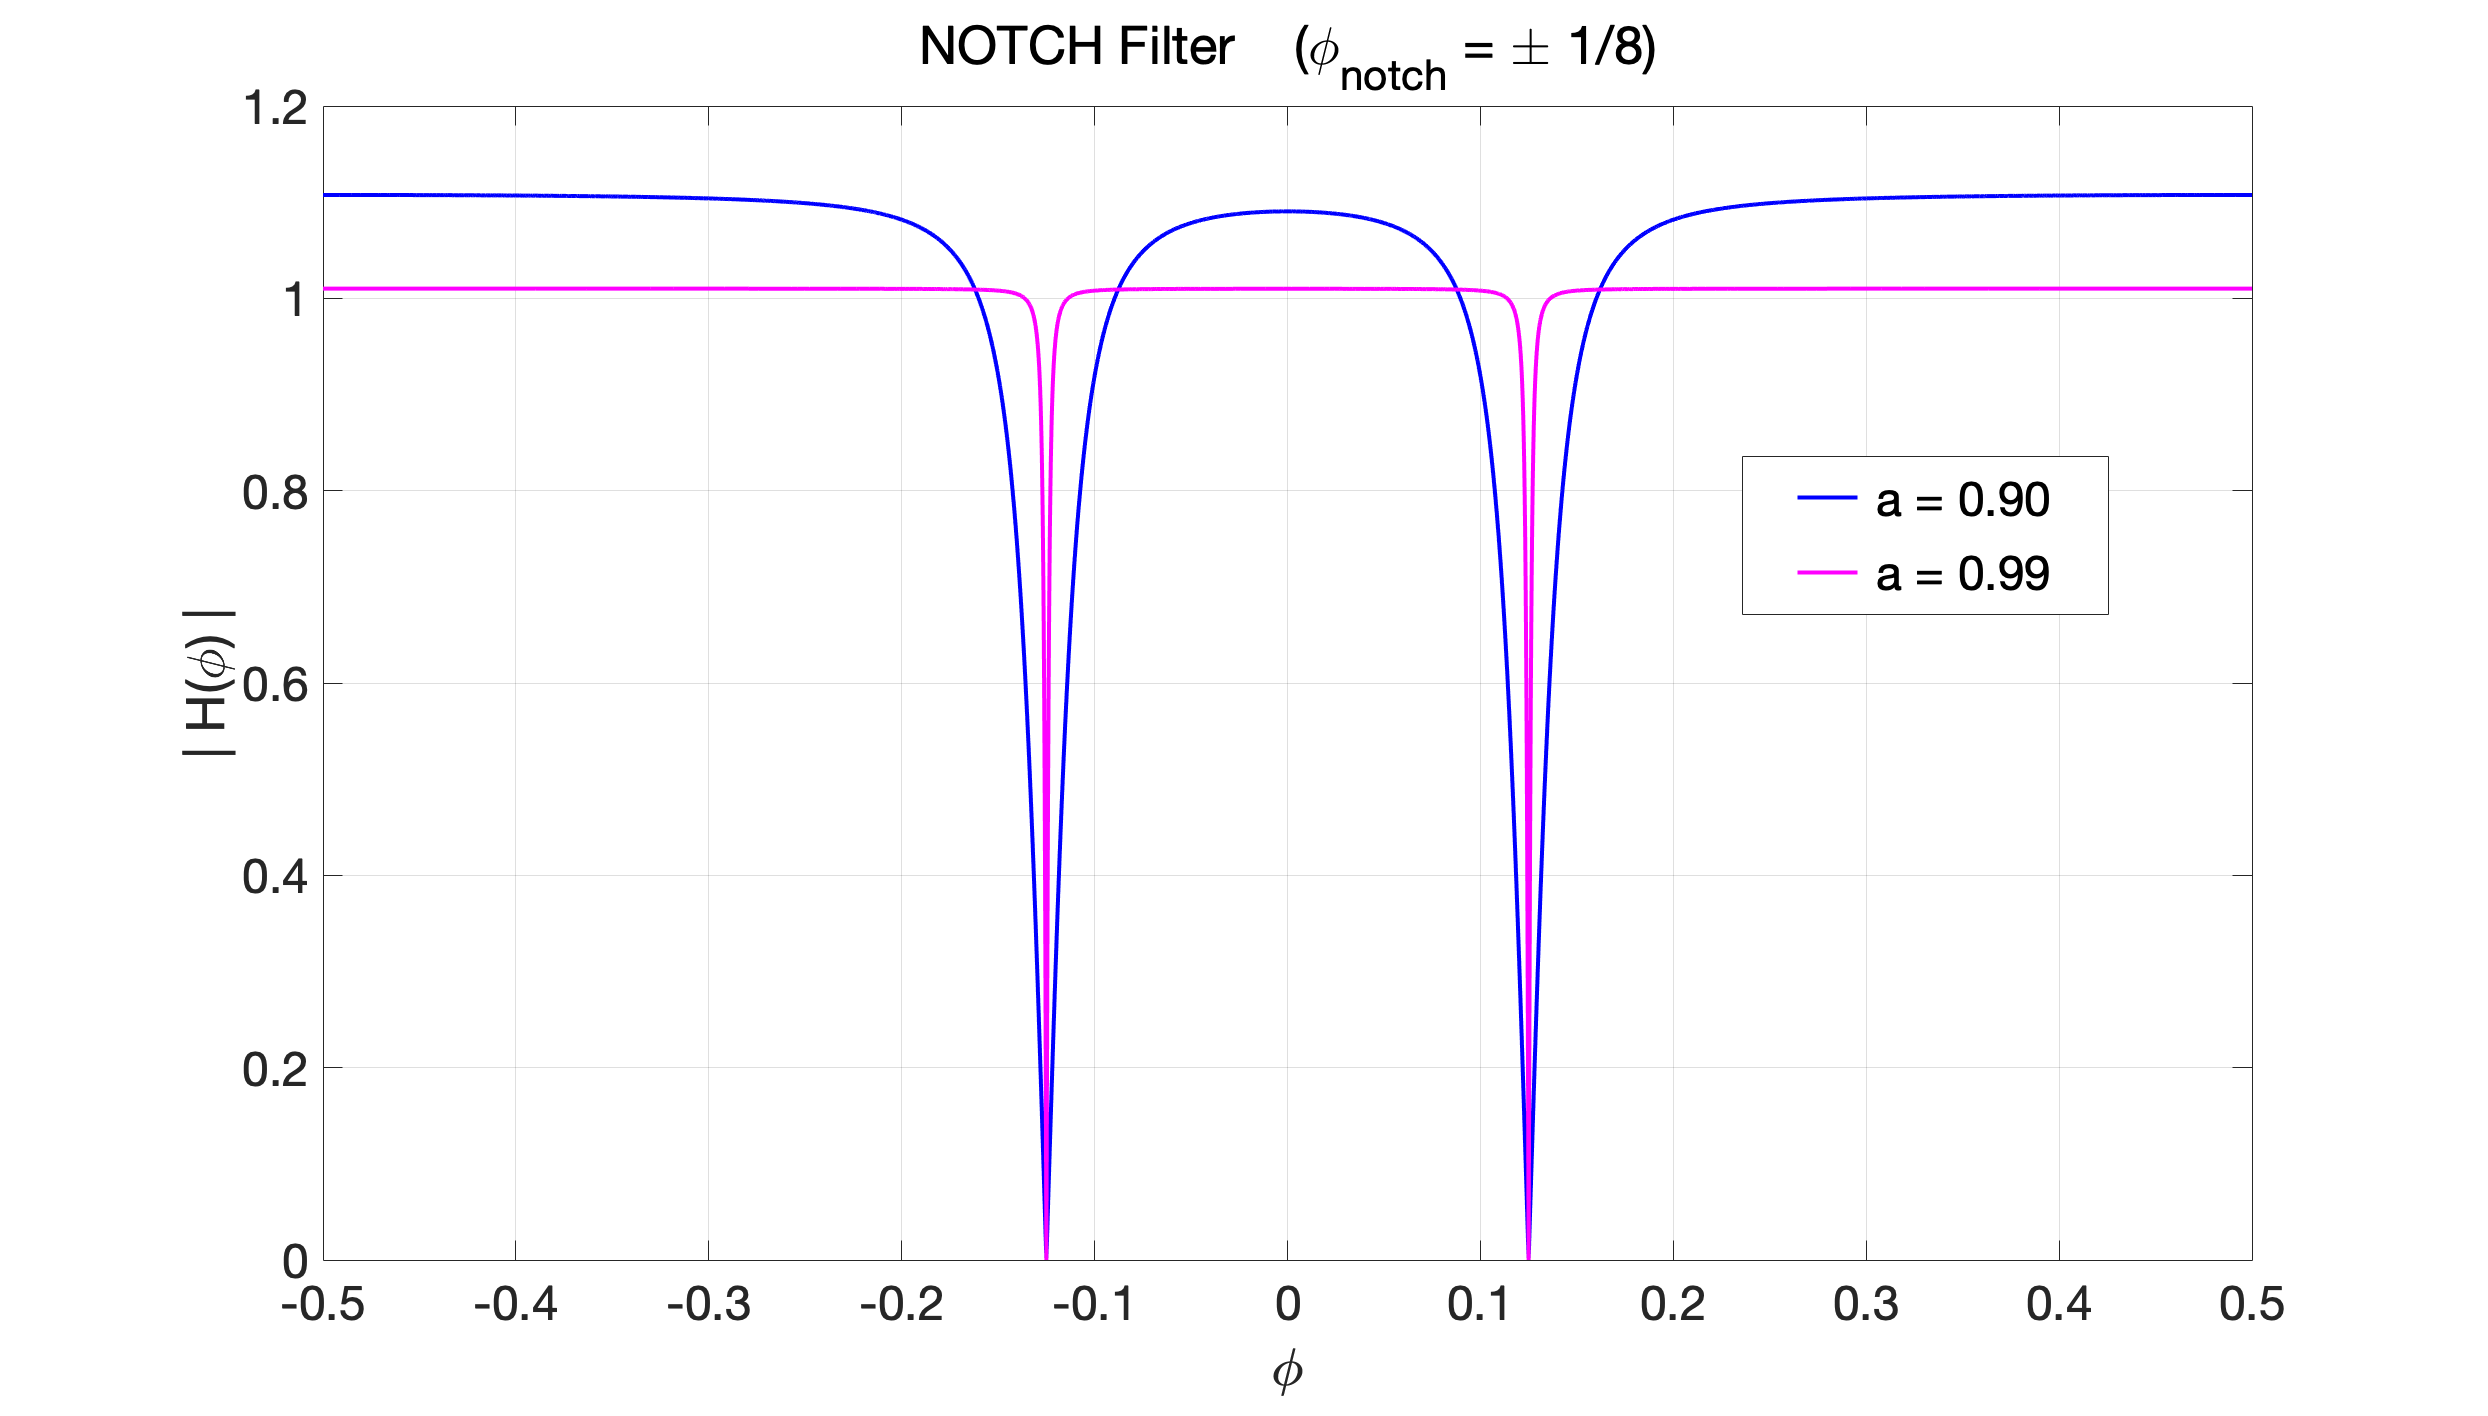
\includegraphics[width=15cm]{src/NotchFilter.png}
\end{document}